%%%%%%%%%%%%%%%%%%%%%%%%%%%%%%%%%%%%%%%%%%%%%%%%%%%%%%%%%%%%%%%%%%%%%%%%%%%%%%%
%%% Describe the IMR model for IMRIs.
%%%%%%%%%%%%%%%%%%%%%%%%%%%%%%%%%%%%%%%%%%%%%%%%%%%%%%%%%%%%%%%%%%%%%%%%%%%%%%%

%
\def\etal{{\it et al.}}  \def\ie{{\it i.e.}}  \def\eg{{\it e.g.}}
\def\lap{\hbox{${_{\displaystyle<}\atop^{\displaystyle\sim}}$}}
\def\gap{\hbox{${_{\displaystyle>}\atop^{\displaystyle\sim}}$}}
\def\lesssim{\mathrel{\hbox{\rlap{\hbox{\lower4pt\hbox{$\sim$}}}\hbox{$<$}}}}
\def\gtrsim{\mathrel{\hbox{\rlap{\hbox{\lower4pt\hbox{$\sim$}}}\hbox{$>$}}}}
\def\alt{\mathrel{\hbox{\rlap{\hbox{\lower4pt\hbox{$\sim$}}}\hbox{$<$}}}}
\def\agt{\mathrel{\hbox{\rlap{\hbox{\lower4pt\hbox{$\sim$}}}\hbox{$>$}}}}
\def\prd{{\it Phys. Rev.} D~}
\def\PRL{{\it Phys.Rev.} Lett~}
\def\apjl{{\it Astrophys. J.} Lett~}
\def\apj{{\it Astrophys. J.}}
\def\Msun{M_\odot}
\def\PRD{{\it Phys. Rev.} D~}
\def\CQG{{\it Class. Quantum Grav.}}
\def\aaps{{\it A\&AS~ }}
\def\pasj{{\it PASJ }}
\def\mnras{{\it MNRAS}} 
\def\aapr{{\it A\&ARv}}

\def\gta{\ifmmode {\mathbin{\lower 3pt\hbox   %> or of order
    {$\,\rlap{\raise 5pt\hbox{$\char'076$}}\mathchar"7218\,$}}}
    \else {${\mathbin{\lower 3pt\hbox
    {$\rlap{\raise 5pt\hbox{$\char'076$}}\mathchar"7218\,$}}}
    $}\fi}
\def\lta{\ifmmode {\,\mathbin{\lower 3pt\hbox   %< or of order
    {$\,\rlap{\raise 5pt\hbox{$\char'074$}}\mathchar"7218\,$}}}
    \else {${\mathbin{\lower 3pt\hbox
    {$\rlap{\raise 5pt\hbox{$\char'074$}}\mathchar"7218\,$}}}
    $}\fi}

%%%%%%%%%%%%%%%%%%%%%%%%%%%%%%%%%%%%%%%%%%%%%%%%%%%%%%%%%%%%%%%%%%%%%%%%%%%%%%%

% \section{Introduction}   
The black hole (BH) mass function in the local Universe is a strongly bi-modal distribution that identifies two main families: stellar-mass BHs with typical masses \(\sim 10M_{\odot}\) observed in Galactic X-ray binaries~\cite{McClintock:2006} and, more recently, in globular clusters~\cite{Morscher:2013}, and supermassive BHs with masses \(\gtrsim 10^{5} M_{\odot}\) observed to be present in most galactic nuclei~\cite{Merloni:2008, Fukugita:2004}.  However, a population of X-ray sources with luminosities in excess of \(10^{39}\, \rm{ erg}\, \rm{s}^{-1} \) has recently been observed, and {\it{Chandra}} and {\it{XMM-Newton}} spectral observations of these ultra-luminous X-ray sources (ULXs) revealed cool disc signatures that were consistent with the presence of intermediate mass BHs (IMBHs) with masses \(10^{2-4} M_{\odot}\)~\cite{Miller:2004,Miller:2004b,Miller:2006_BOOK}. Subsequent observations have shown that these ULXs have spectral and temporal signatures that are not consistent with the sub-Eddington 
accretion regime that is expected for IMBHs at typical ULX luminosities. Rather, these later studies suggest that many ULXs are powered by super-Eddington accretion onto \(\lesssim 100 M_{\odot}\) BH remnants.  Nevertheless, recent work by Swartz et al.~\cite{Swartz:2011} demonstrates that there is a subpopulation of ULXs that seem to be powered by a separate physical mechanism. These objects have typical luminosities \(L\gtrsim 10^{41}\, \rm{ erg}\, \rm{s}^{-1} \), which cannot be explained by close to maximal radiation from super-Eddington accretion onto massive BHs formed in low metallicity regions~\cite{Zampieri:2009, Belczynski:2010, Ohsuga:2011}. Several hyper-luminous X-ray sources, including M82 X-1, ESO 243-49 HLX-1, Cartwheel N10 and CXO J122518.6+144545, present the best indirect evidence for the existence of IMBHs~\cite{Matsumoto:2001,Farrel:2009,Wolter:2010,Jonker:2010}.  In particular, the colocation of M82 X-1 with a 
massive, young stellar cluster, the features of its power spectrum, and some reported transitions between a hard state and a thermal dominant state, make this object a strong IMBH candidate~\cite{Portegies:2004,Strohmayer:2003,Kaaret:2007,Feng:2010}.  Recent searches of archival {\it{Chandra}} and {\it{XMM-Newton}} data sets have also uncovered two new hyper-luminous X-ray sources with luminosities in excess of \(10^{39}\, \rm{ erg}\, \rm{s}^{-1} \). These sources are the most promising IMBH candidates currently known, although the highest possible super-Eddington accretion rate onto the largest permitted BH remnant cannot yet be ruled out~\cite{Sutton:2012}.  This increasing body of observational evidence~\cite{Trenti:2006,Coleman:2004}, and the fact that the existence of IMBHs provides a compelling explanation for the initial seeding of supermassive BHs present in most galactic nuclei~\cite{Volonteri:2010,Schneider:2002,Yu:2002} has revived the quest for these elusive objects.  

A promising channel for detection of IMBHs is through the emission of gravitational radiation during the coalescence of stellar-mass compact remnants --- neutron stars (NSs) or BHs --- with IMBHs in core-collapsed globular clusters. This expectation is backed up by numerical simulations of globular clusters~\cite{Taniguchi:2000,Miller:2002,Mouri:2002a,Mouri:2002b,Gultekin:2004,Gultekin:2006,Oleary:2006,Oleary:2007}  which suggest that IMBHs could undergo several collisions with stellar-mass compact remnants during the lifetime of the cluster through a variety of mechanisms, including gravitational radiation, Kozai resonances and binary exchange processes.  As discussed in~\cite{man}, the most likely mechanism for the formation of binaries involving a stellar-mass compact remnant and an IMBH is hardening via three body interactions, with an expected detection rate of \(\sim 1-10\, {\rm{yr}}^{-1}\) with ground-based observatories~\cite{man,Abadie:2010}. 


% Since hyper-luminous X-ray sources are rare, and our knowledge about their astrophysical properties is still limited, we may have to use a different means to search for IMBHs in order to improve our knowledge about the channels that lead to the formation of these objects, and to shed light on their astrophysical properties, such as mass and spin distributions~\cite{mandel}. 
% In this chapter we explore the use of observations in the gravitational wave (GW) spectrum to gain insight into the properties of IMBHs. 
% 
The current upgrade of the LIGO and Virgo detectors~\cite{aLIGO, virgo}, will enable the detection of IMBHs with masses \(50 M_{\odot} \lesssim M \lesssim 500 M_{\odot}\), by achieving their target sensitivity at low-frequencies down to 10Hz~\cite{ZDHP:2010}.  Advanced LIGO (aLIGO) and Advanced Virgo are expected to have greatest sensitivity in the 15Hz - 1kHz range, with a peak at \(\sim60\) Hz (see Figure~\ref{ZDHP_promise}). 
% Proposed third generation detectors, such as the Einstein Telescope~\cite{Freise:2009}, aim to extend the frequency range of ground-based detectors down to 1Hz, in order to search for GWs emitted by binaries of \(10^{2-4}M_{\odot}\) BHs~\cite{etgair,Huerta:2011a,Huerta:2011b}. 
% 
% 
\begin{figure*}[ht]
\centerline{
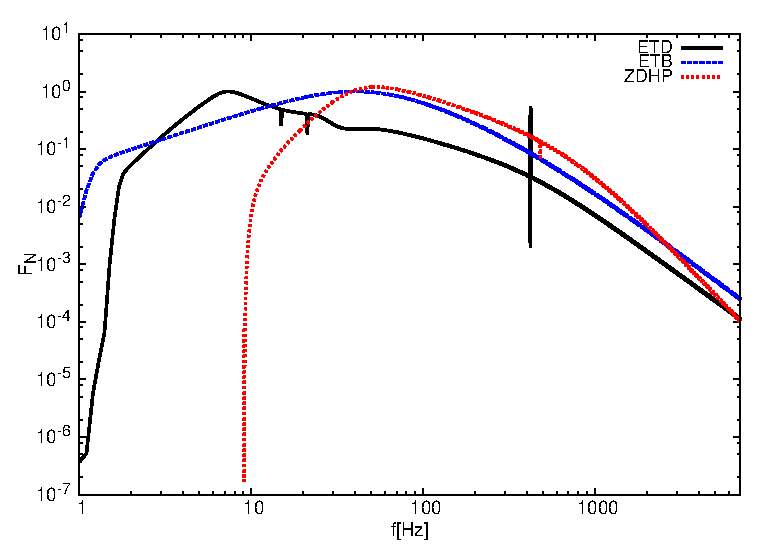
\includegraphics[height=0.6\columnwidth,  clip]{figures/imrimri/nc_normalized.eps}
}
\caption{The panel shows the expected sensitivity for two configurations of the Einstein Telescope (ET), namely, ETD (black), ETB (blue) and LIGO's Zero Detuned High Power (ZDHP) configuration (red). The vertical axis measures \(F_{\rm{normalized}} =  \left(f/f_{\rm{max}}\right)^{-7/6}\sqrt{S_n(f_{\rm{max}})/S_n(f)}\), where \(f_{\rm{max}}\) is the maximum of the corresponding power spectral density, \(S_n(f)\).
}
\label{ZDHP_promise}
\end{figure*}
% 
% 
The frequency of the dominant quadrupolar harmonic in the GWs emitted at the
innermost stable circular orbit (ISCO) for a binary of non-spinning objects is 
\begin{equation}
f_{\rm{ISCO}}= 4.4 {\rm{kHz}} \left(\frac{M_{\odot}}{M}\right).
\label{fIMRIisco}
\end{equation}
For a typical intermediate mass--ratio coalescence (IMRC) with total mass 
\(M\gtrsim 100 M_{\odot}\), advanced detectors will observe the late inspiral,
merger and ringdown; with the latter two phases contributing significantly to the 
overall SNR~\cite{Smith:2013}.
% However, the heaviest IMRCs, with masses $\gtrsim500M_\odot$, will coalesce at or below the low frequency limit of the bandwidth. 
% Hence, merger and ringdown will significantly contribute to the SNR of IMRCs over a considerable portion of the detectable mass-range~\cite{Smith:2013}. 
In order to maximize the science output of GW observations of IMRCs, it is 
therefore necessary to model the inspiral, merger and ringdown consistently. 
% In order to make progress in this direction, we previously developed a waveform model that combined results from Black Hole 
% Perturbation Theory (BHPT) and post-Newtonian (PN) theory to  explore the information that could be obtained from observations of IMRCs with the EinsteinTelescope~\cite{Huerta:2011a,Huerta:2011b}. Although this model provided an important step in exploring the science that could be done with IMRC observations, the model was limited.
% 
% 
% In previous work~\cite{Huerta:2012zy}% and in~\cite{Huerta:2009,Huerta:2010,Huerta:EHE,Huerta:2012}
% we explored using the self-force formalism~\cite{SFB,LRP} to develop a waveform model with a robust description of the dynamical evolution of IMRCs during the inspiral phase. These were found to be effective when used to carry out matched-filter based searches for inspiral-only IMRCs~\cite{Smith:2013}, but searches for IMRCs in the advanced detector era will require waveform models that include not only the inspiral but also the merger and ringdown~\cite{Smith:2013}. The model described in~\cite{Huerta:2011a} included merger and ring down but without the self-force driven inspiral.
While modeling of IMRCs would benefit greatly from NR simulations, simulating
mergers for mass-ratios%
\footnote{Note that the definition of mass-ratio $q$ is different from the
previous chapters, where $q\geq 1$. We choose the definition with $q\leq 1$ here
to ensure that in the extreme mass-ratio regime $q\rightarrow 0$
as $\eta\rightarrow 0$. See Section~\ref{ssec:nomenclature}.}
% 
 \(q=m_1/m_2 \lesssim 1/10\) are prohibitively computationally expensive at
present~\cite{Mroue:2013xna}. On the other hand, recent 
% breakthroughs in the self-force program that have 
results show that the conservative part of self-force can reproduce
results from NR simulations of comparable-mass binary systems~\cite{LeTiec:2012}.  
Furthermore, the recent computation of the self-force inside the ISCO 
equips us to develop models that better reproduce the strong field dynamics of 
BH binaries~\cite{Akcay:2012}.  

\begin{figure*}%[ht]
\centerline{
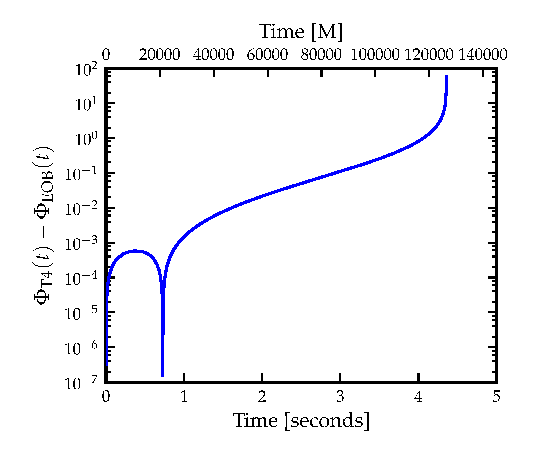
\includegraphics[height=0.45\columnwidth,  clip]{figures/imrimri/m1m006_phasedifftM_T4EOB_r030tM.eps}
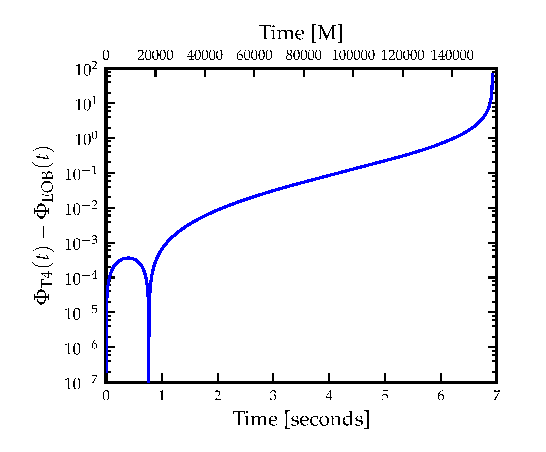
\includegraphics[height=0.45\columnwidth,  clip]{figures/imrimri/m1m008_phasedifftM_T4EOB_r030_tM.eps}
}
\centerline{
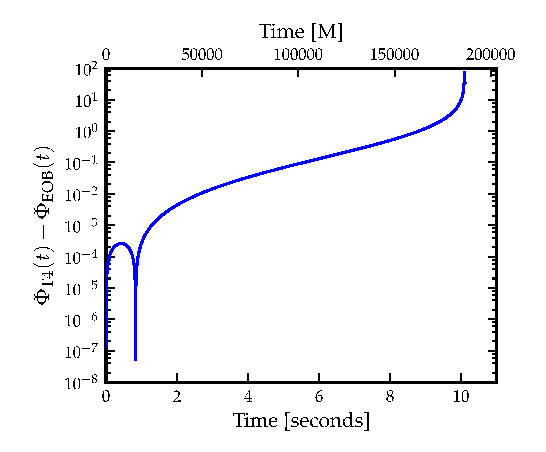
\includegraphics[height=0.45\columnwidth,  clip]{figures/imrimri/m1m010_phasedifftM_T4EOB_r030tM.eps}
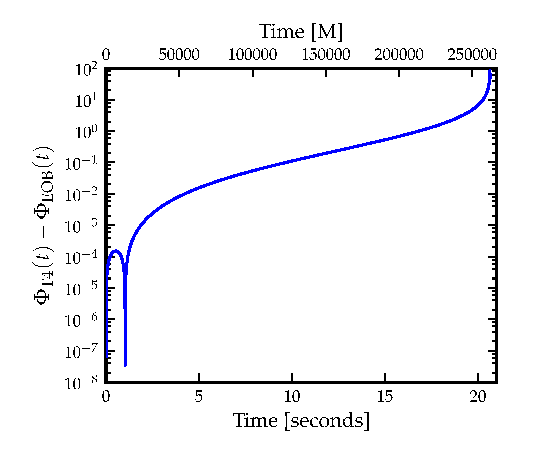
\includegraphics[height=0.45\columnwidth,  clip]{figures/imrimri/m1m015_phasedifftM_T4EOB_r030_tM.eps}
}
\caption{The phase discrepancy in radians between the PN approximant TaylorT4, and the Effective One Body model, shown as a function of time from \(r=30M\) to the point when the TaylorT4 model reaches the ISCO. The systems have mass-ratio, $q$, total mass, \(M\), and final phase discrepancy, $\Delta\Phi$: $(q, M, \Delta\Phi) = (1/6, 7M_{\odot},21.5\,{\rm rads})$ (top-left), $(1/8, 9M_{\odot},30.2\,{\rm rads})$ (top-right), $(1/10, 11M_{\odot},70.1\,{\rm rads})$ (bottom-left) and $(1/15, 16M_{\odot},83.2\,{\rm rads})$ (bottom-right) respectively.}
\label{pn_approx}
\end{figure*}


In this chapter we combine recent developments in the self-force program, in 
PN theory and in NR to develop a model that describes the inspiral, merger and
ringdown of IMRCs and comparable mass-ratio systems. In Section~\ref{ssec:inspiral} 
we
discuss the modelling of the conservative part of the self-force during inspiral.
Using \(\mathcal{O}(\eta)\)\footnote{\(\eta=m_1 m_2/(m_1+m_2)^2\)} 
self force results for binaries with mass-ratios \(q\gtrsim1/6\) gives a 
system without an ISCO. We discuss the implications of this result for 
the modeling of comparable and intermediate mass--ratio binaries.  
% 
In Section~\ref{ssec:dissipative}, we describe our approach 
to model the radiative part of the self-force for the inspiral evolution. 
% 
In Section~\ref{trans}, we extend the transition scheme of 
Ori and Thorne~\cite{ori} by including finite mass-ratio corrections, and model
the orbital phase evolution using the implicit rotating source (IRS) model. 
We adopt the IRS description for the late-time radiation in order to provide a 
smooth progression from late inspiral to ringdown, as it provides the correct 
orbital frequency evolution in the vicinity of the light-ring. 
% 
Finally, in Section~\ref{RDwav} we construct the ringdown waveform using a 
sum of quasinormal modes. Section~\ref{conclu} presents a summary of our 
findings and future directions of work. 

In addition to IMBH--BH binaries, NS--BH binaries also have mass-ratios 
\(q \lesssim 1/6\). NSBH mergers are promising GW sources for second generation detectors
with an estimated detection rate of \(0.2-300\) mergers a year~\cite{LSCCBCRates2010}. 
Past GW searches for NSBH systems used PN waveforms as templates, which have
been demonstrated to be insufficiently accurate for aLIGO searches~\cite{Nitz:2013mxa}. 
In Figure~\ref{pn_approx}, we show the phase difference between the PN approximant TaylorT4~\cite{TaylorT4Origin} and the EOB model introduced
in~\cite{BuonannoEOBv2Main}. The model we develop here would 
also be applicable to NSBH detection searches.



\section{Modeling}
\label{one}


\subsection{Nomenclature}\label{ssec:nomenclature}
Throughout this chapter we will use units with \(G=c=1\), unless otherwise stated. We consider BH  binaries on circular orbits with component masses \(m_1, m_2\), such that \(m_1 < m_2\). We assume that the binary components are non spinning. We use several combinations of the masses in the following sections, which are summarized in Table~\ref{length}. 

\begin{table}[thb]
\centering
\begin{tabular}{|c| c| }
\hline
\multicolumn{2}{|c|}{Binary masses}  \\\cline{1-2} 
\(m_1\) & mass of inspiralling compact object  \\ [0.7ex] 
\(m_2 \) & mass of central compact object  \\ [0.7ex]  
\(M=m_1+m_2 \) & total mass of binary system \\ [0.7ex]  
\(q=\frac{m_1}{m_2} \) & (with $m_1\leq m_2$) mass--ratio \\ [0.9ex]  
\(\mu=\frac{m_1 m_2}{m_1 + m_2} \) & reduced mass \\ [0.9ex]  
\(\eta= \frac{\mu}{M}\) & symmetric mass--ratio \\ [0.9ex]  
\hline
\end{tabular}
\caption{The table summarizes the nomenclature we will use throughout our analysis.}
\label{length}
\end{table}

Note that the definition of the mass-ratio $q$ is different from the previous chapters, where
$q\geq 1$. We choose the definition with $q\leq 1$ here to ensure that in the 
extreme mass-ratio regime both $q\rightarrow 0$ and $\eta\rightarrow 0$.
% Having defined the variables to be used in the subsequent sections, we shall now describe the construction of the self-forced waveform model. The model consists of four building blocks --- the inspiral, the transition, the plunge and the ringdown phases. The next section describes the inspiral evolution. 

\subsection{Inspiral evolution}
\label{ssec:inspiral}
We model the inspiral phase evolution in the context of the Effective One Body  (EOB) formalism~\cite{EOB:Damour}, i.e., we consider the scenario in which the dynamics of a binary system is mapped onto the motion of a test particle in a time-independent and spherically symmetric Schwarzschild space-time with total mass \(M\):
\begin{equation} 
\mathrm{d}s^{2}_{\rm{EOB}} = -A(r)\mathrm{d}t^2 + B(r)\mathrm{d}t^2 + r^2\mathrm{d}\Omega^2\,,
\label{metricEOB}
\end{equation} 
\noindent where the potentials \(A, \, B\) are known to 3PN order~\cite{Buonanno:1999,Damour:2000}. In the test-mass particle limit \(\eta\rightarrow 0\), these potentials recover the Schwarzschild results, namely:
\begin{equation}
A(u, \eta\rightarrow 0) = B^{-1}(u,  \eta\rightarrow 0)= 1-2\,u,\quad {\rm{with}} \quad u=\frac{M}{r}.
\label{limitEOB}
\end{equation}
\noindent In the EOB formalism, the orbital frequency evolution can be
derived from the Hamiltonian, \(H_{\rm{EOB}}\)~\cite{EOB:Damour},
\begin{equation} 
H_{\rm{EOB}} = M\sqrt{1+2\,\eta\left(H_{\rm{eff}} -1\right)},
\label{EOBH}
\end{equation}
\noindent using the Hamiltonian equation:
\begin{equation}
\frac{d \phi}{d \mathrm{t} } =  M\Omega = \frac{\partial H_{\rm{EOB}}}{\partial L} = \frac{u^2\,L(x)\,A(u)}{H(u)\,H_{\rm{eff}}(u)},
\label{new_phase}
\end{equation}
\noindent where 
\begin{eqnarray}
H_{\rm{eff}}(u) = \frac{A(u)}{\sqrt{\tilde{A}(u)}}\,, \qquad  \tilde{A}(u)= A(u) + \frac{1}{2}\,u\,A'(u),     \qquad H(u)=\dfrac{H_{\rm{EOB}}}{M},\\\nonumber
\label{params_for_new_phase}
\end{eqnarray}
$(')$ denotes $\pd_u$, and $L$ is the binary's orbital angular momentum.
Recent work has enabled the derivation of gravitational self-force corrections 
to the EOB potential \(A(u)\rightarrow  1-2u+\eta\, a(u) + {\cal{O}}(\eta^2)\)~\cite{barus}.
Deriving this gravitational self-force contribution,  \(a(u)\), is equivalent to 
including all PN corrections to the EOB potential \(A(u)\) at linear order in 
\(\eta\). We shall now briefly describe the construction of the 
gravitational self-force contribution \(a(u)\), emphasizing the fact that this
contribution encodes information about the strong-field regime of the gravitational field. 

As shown by Detweiler and Whiting~\cite{Detweiler:2003}, the gravitational self-force corrected worldline can be interpreted as a  geodesic in a smooth perturbed spacetime with metric
 \begin{equation}
 g_{\alpha \beta} =  g^{0}_{\alpha \beta}(m_2) + h^{R}_{\alpha \beta},
 \label{detint}
 \end{equation}
where the regularized \(R\) field is a smooth perturbation 
associated with \(m_1\). Detweiler proposed the gauge invariant 
``redshift observable'' \(z_1\) to handle the conservative effect of the gravitational
self-force in circular motion~\cite{Detweiler:2008,Detweiler:2009}.
\(z_1\) can be interpreted as the gravitational red-shift of 
light rays emitted from the smaller compact object, and received far
away from the binary along the direction perpendicular to the
orbital plane~\cite{Detweiler:2008}.
 \begin{equation}
z_1(\Omega)= \sqrt{1-3x}\left(1- \frac{1}{2} h^{R,\,F}_{uu} + q \frac{x}{1-3x}\right),
\label{detinv}
\end{equation}
\noindent where  \(x\) is the gauge-invariant dimensionless frequency parameter 
given by \(x=\left(M \Omega\right)^{2/3}\), \(h^{R,\,G}_{uu}\) is a double
contraction of the regularized metric perturbation with the four-velocity
\(u^{\mu}\), i.e. \( h^{R,\, G}_{uu} = h^{R,\,G}_{\mu\nu}u^{\mu} u^{\nu} \), 
where the label \(G\) indicates the gauge used to evaluate the metric perturbation.
The label \(F\) in Eq.~\ref{detinv} indicates that it is valid within the class 
of asymptotically {\it F}lat gauges.
In a convenient gauge, the redshift coincides with the 
inverse time components of the four-velocities \(u^\alpha\) of the
component, namely \(z_1 = 1/u^t_1\)~\cite{Detweiler:2008}.
In~\cite{Akcay:2012}, \(z_1(\Omega)\) was calculated in the Lorenz gauge and the 
following gauge transformation can be used to link the asymptotically flat 
\(h^{R,\,F}_{uu} \) metric perturbation to its Lorenz-gauge counterpart 
\(h^{R,\,L}_{uu} \):
\begin{equation}
h^{R,\,F}_{uu} = h^{R,\,L}_{uu} + 2q\frac{x(1-2x)}{\left(1-3x\right)^{3/2}}.
\label{flgauge}
\end{equation}
Hence, inserting Eq.~\eqref{flgauge} into Eq.~\eqref{detinv} leads to
 \begin{equation}
z_1(\Omega)= \sqrt{1-3x}\left(1- \frac{1}{2} h^{R,\,L}_{uu}  - 2q\frac{x(1-2x)}{\left(1-3x\right)^{3/2}} + q \frac{x}{1-3x}\right).
\label{detinvLOR}
\end{equation}
The EOB potential \(a(x)\) can be constructed from $h_{uu}^{R,L}$ via
\begin{equation}
 a(x) = -\frac{1}{2}\left(1-3x\right)\tilde{h}^{R,\,L}_{uu} - 2x \sqrt{1-3x},
 \label{formal_a}
 \end{equation}
 \noindent with \(\tilde{h}^{R,\,L}_{uu}= q^{-1}h^{R,\,L}_{uu}\). 
 In~\cite{Akcay:2012} accurate numerical data is obtained for \(h^{R,\,L}_{uu}\)
in the Lorenz gauge. Using the above relation, Ref.~\cite{Akcay:2012} 
provides a useful fit formula for \(a(x)\) that is valid over the range 
\(0 < x < \frac{1}{3}\), 
 \begin{equation}
 a(x)= 2x^3\, \frac{(1-2x)}{\sqrt{1 - 3 x}}\,a_{E}(x),
 \label{pot}
 \end{equation}
where \(a_E(x)\) is given in Eq.~(54) of~\cite{Akcay:2012}.
% Using the above dictionary, the model for \(a(x)\) in this chapter 
% reproduces \(a_{E}(x)\) 
% to within a maximal absolute difference of \(1.2\times10^{-5}\) for 
% \(0<x<\frac{1}{3}\). 
Using the phenomenological fit for the function $a(x)$, the self-force
corrected energy and angular momentum are given by~\cite{Akcay:2012, barus}
{\allowdisplaybreaks\begin{align}\label{enofxeq}
E(u(x)) &= E_0(x) +  \eta\left(-\frac{1}{3}\frac{x}{\sqrt{1-3x}}a'(x) + \frac{1}{2}\frac{1-4x}{\left(1-3x\right)^{3/2}} a(x) - \right.\nonumber\\
& \hspace{20mm} \left. E_0(x)\left( \frac{1}{2}E_0(x) + \frac{x}{3}\frac{1-6x}{\left(1-3x\right)^{3/2}} \right)\right),\\
\label{lzofxeq}
L (u(x)) &= L_0(x) +  \eta\left( -\frac{1}{3}\frac{x}{\sqrt{x(1-3x)}}a'(x) -\frac{1}{2}\frac{1}{\sqrt{x}\left(1-3x\right)^{3/2}} a(x)  \right.\nonumber\\
& \hspace{20mm} \left. -\frac{1}{3 }\frac{1-6x}{ \sqrt{x} \left(1-3x\right)^{3/2}}\left(E_0(x)-1\right)  \right)\,,\\
\label{rofx}
{\rm{with}} \quad u(x)&= x\left( 1+ \eta\Bigg[\frac{1}{6}a'(x) + \frac{2}{3}\left(\frac{1-2x}{\sqrt{1-3x}} -1 \right) \Bigg] \right)\,,
\end{align}}
where \((')\) denotes \(\pd_x\), and \(E_0(x)\) and \(L_0(x)\) are given by
\begin{eqnarray}
E_0(x) &=&  \frac{1-2x}{\sqrt{1 - 3 x}} -1,\\
\label{enofx_0}
L_0(x)&=&   \frac{1}{\sqrt{x (1 - 3 x)}}.
\label{lzofx_0}
\end{eqnarray}
   
\begin{figure*}%[ht]
% \centerline{
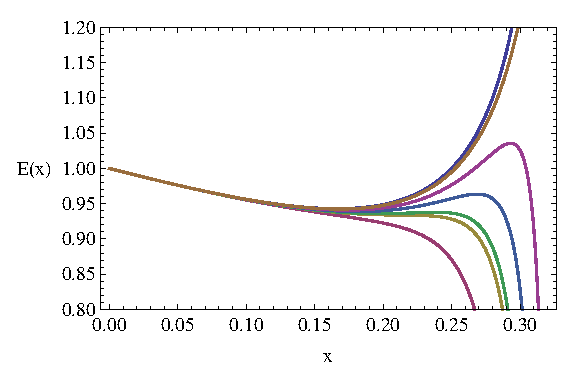
\includegraphics[height=0.6\columnwidth,  clip]{figures/imrimri/eofx.eps}
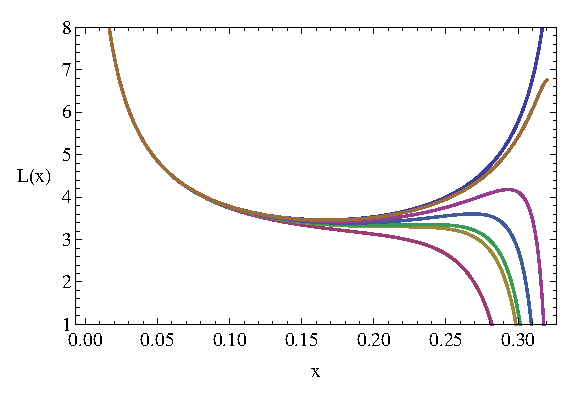
\includegraphics[height=0.6\columnwidth,  clip]{figures/imrimri/lofx.eps}
% }
\caption{The panels show the energy and angular momentum given by Eqs.~\eqref{enofxeq}-\eqref{lzofxeq}, respectively. We show the functional form of these parameters for binary systems with mass-ratio values, from top to bottom, \(q \in [0,\, 1/100, \,1/20, \,1/10, \,1/6, \,1/5, \,1 ]\).  }
\label{orbitalparams}
\end{figure*}

\noindent In Figure~\ref{orbitalparams}, we  show the effect of these conservative corrections on the orbital parameters.


As discussed in~\cite{barus}, minimizing the self-force corrected energy,
given by Eq.~\eqref{enofxeq}, with respect to the orbital frequency, predicts
that binary systems with mass-ratios \(q\in \{1, \,1/2, \,1/3\}\) do not have
an ISCO. 
It was argued in~\cite{barus} that deriving self-force results in the strong
field regime may alleviate this problem. We explored this issue, and found
that using linear--in--\(\eta\) self-force corrections does not fix this
problem for comparable mass-ratio systems. 
In Figure~\ref{dedx}, we show that the existence of an ISCO is guaranteed 
for BH binaries with symmetric mass-ratio 
\(\eta\lesssim 6/49\, ({\rm{or}}\, q \lesssim 1/6)\), and its location may
be approximated by
\begin{equation}
x_{\mathrm{ISCO}}=\frac{1}{6}\left(1+ 0.83401\eta+4.59483\eta^2\right).
\label{xisco_eq}
\end{equation}
It remains to be seen whether the inclusion of \(\mathcal{O}(\eta^2)\)
conservative corrections gives an ISCO for binaries with 
mass-ratios \(q\gtrsim 1/6\). 

 
\begin{figure*}%[ht]
\centerline{
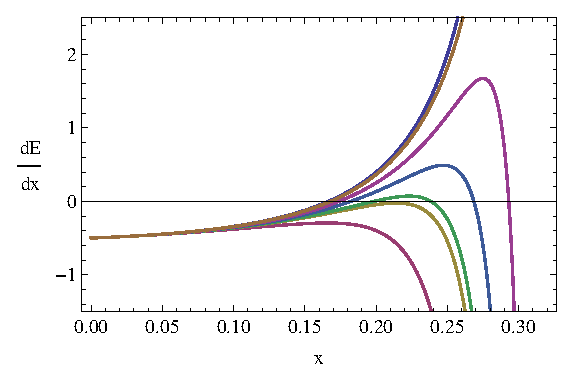
\includegraphics[height=0.6\textwidth,  clip]{figures/imrimri/dedx_for_isco.eps}
}
\caption{The location of the innermost stable circular orbit is determined by the condition \({\rm{d}}E/\rm{d}x = 0\). The panel shows \({\rm{d}}E/\rm{d}x\) as a function of the gauge invariant quantity \(x=\left(M\,\Omega\right)^{2/3}\). The various curves represent binary systems with mass-ratios, from top to bottom, \(q \in [0,\, 1/100, \,1/20, \,1/10, \,1/6, \,1/5, \,1 ]\). Note that binaries with mass-ratios \(q\gtrsim 1/6\) do not have an ISCO in this model. }
\label{dedx}
\end{figure*}

In summary, the building blocks to construct the conservative dynamics are

\begin{itemize}
\item The orbital frequency evolution is computed using Eq.~\eqref{new_phase} with the gravitational self-force contribution included in the potential \(A(u)= 1-2u + \eta\, a(u)\).
\item Eq.~\eqref{new_phase} is evaluated using the self-force-corrected expression for the angular momentum, \(L(x)\), given by Eq.~\eqref{lzofxeq}. The self-force-corrected expression for the energy, given in Eq.~\eqref{enofxeq} is only used to determine the point at which the inspiral ends and the transition region begins.
\end{itemize}

Eq.~\eqref{new_phase} accurately models the orbital frequency from early 
inspiral through the ISCO. However, the post-ISCO time evolution of this 
prescription does not render an accurate representation of the orbital 
frequency as compared to numerical relativity simulations. 
This problem was addressed in the EOB formalism by introducing the 
phenomenological non-quasi-circular coefficients~\cite{BuonannoEOBv2Main}.
The approach we follow to circumvent this problem is described
in Section~\ref{trans}.

This completes the description of the conservative part. We now describe how to couple this with the radiative part of the self-force to model the inspiral evolution. 
 
 \subsection{Dissipative dynamics}
\label{ssec:dissipative}
A consistent self-force evolution model that incorporates first-order
in mass-ratio conservative  corrections should also include second-order
radiative corrections. However, second-order self-force radiative 
corrections are not known at present. 
% Several studies have demonstrated 
% the importance of including the missing second order corrections to the
% radiative part of the self-force, both for source detection and for parameter estimation~\cite{Isoyama:2013, Burko:2012, Huerta:2012, Huerta:2010, Huerta:2009}. 
% 
We use a new prescription for the energy flux that includes PN 
corrections up to \(22^\mathrm{nd}\) PN order~\cite{Fujita:2012},
\begin{eqnarray}
\label{enfluxpn}
\left(\dot E\right)_{\rm PN}
&=& -\frac{32}{5}\frac{\mu^2}{M}x^{7/2}\Bigg[1-\frac{1247}{336}x + 4\pi x^{3/2}  - \frac{44711}{9072}x^2-\frac{8191}{672}\pi x^{5/2}  \\\nonumber 
&+&x^3 \bigg\{\frac{6\,643\,739\,519}{69\,854\,400} +\frac{16}{3}\pi^2 -\frac{1712}{105}\gamma_{\rm E} -\frac{856}{105}\ln(16x) \Big\} -\frac{16285}{504} \pi x^{7/2} \\\nonumber
&+&  x^4 \Big\{-\frac{323105549467}{3178375200}  + \frac{232597}{4410}\gamma_{\rm E} -\frac{1369}{126}\pi + \frac{39931}{294}\ln(2)  \\\nonumber
&-&\hspace{20mm}\frac{47385}{1568}\ln(3)  +\frac{232597}{4410}\ln(x) \Big\}  \\\nonumber 
&+&  x^{9/2}\Big\{ \frac{265978667519}{745113600}\pi -\frac{6848}{105}\gamma_{\rm E}\pi -\frac{13696}{105}\pi\ln(2)  -\frac{6848}{105}\pi\ln(x)\Big\} \\\nonumber
&+& {\rm{ higher \, order \, corrections \, up\, to \, 22PN \, order}} \Bigg],
\end{eqnarray}
and include the \(\mathcal{O}(\eta)\) corrections through the exponential
resummation approach of~\cite{Isoyama:2013}. In this approach, the energy flux is
\begin{eqnarray}
\left(\frac{{\mathrm{d}}E}{{\mathrm{d}}t}\right)_{\rm hybrid} &=& {\cal{L}}_{\rm 0} \exp\left( {\cal{L}}_{\eta} \right)\, ,
\label{pnfluxfit}
\end{eqnarray}
\noindent where \( {\cal{L}}_{\rm 0} \) denotes the leading-order in mass-ratio PN energy flux given in Eq.~\eqref{enfluxpn}, and \( {\cal{L}}_{\eta} \) incorporates mass-ratio corrections to the highest PN order available~\cite{Joguet:2002,Buonanno:2011_tail,Isoyama:2013}, and additional corrections characterised by a set of unknown coefficients,  \(b_i\) 
\begin{eqnarray}
\label{etacorrect}
{\cal{L}}_{\eta} 
&=& \Bigg[x\bigg[-\frac{35}{12}\eta + b_1\,\eta^2\bigg] + 4\pi x^{3/2}\bigg[ b_2\, \eta + b_3 \eta^2 \bigg]  + x^2 \bigg[\frac{9271}{504}\eta + \frac{65}{18}\eta^2\bigg]  \\\nonumber
&+& \pi x^{5/2}\bigg[ -\frac{583}{24} \eta + b_4\, \eta^2\bigg] + x^3 \bigg[\eta\left(-\frac{134\,543}{7\,776} + \frac{41}{48}\pi^2\right) -\frac{94403}{3024}\eta^2 - \frac{775}{324}\eta^3\bigg] \\\nonumber
&+&  \pi x^{7/2} \bigg[\frac{214745}{1728} \eta +  \frac{193385}{3024}\eta^2\bigg]   \Bigg].
\end{eqnarray}
\noindent  The coefficients \(b_i\) were taken to be constant 
in~\cite{Isoyama:2013}, but we found that a better match to the EOB phase
evolution could be obtained by allowing an additional dependence on mass-ratio
in these terms (see Eqs.~\eqref{B1}-\eqref{B3} below).  We constrain the 
\(b_i\) coefficients by ensuring that the resulting phase evolution  
reproduces the phase evolution predicted by the EOB model introduced 
in~\cite{BuonannoEOBv2Main, Damour:2013}, which was calibrated to NR 
simulations of comparable mass binaries. 
To do so, we implemented the EOB model~\cite{BuonannoEOBv2Main} and performed
a Monte Carlo simulation to optimize the values of the \(b_i\) coefficients 
(see Figure~\ref{bimaps}). The optimization was done in two stages. We 
started by considering the three coefficients \(b_1,\, b_2\) and \(b_4\),  
sampling a wide range of parameter space, namely \(b_i\in[-200,200]\).
We constrained the duration of the waveform from early inspiral to the 
light-ring to be similar to its EOB counterpart. Waveforms that differed from
their EOB counterparts by more than \(10^{-4}\) seconds in duration were
discarded. Once the region under consideration had been sparsely sampled, we
focused on regions of parameter space where the orbital phase evolution was
closest to the EOB evolution, and finely sampled these to obtain the optimal 
values for the coefficients. We found that this approach enabled us to 
reproduce the EOB phase evolution with a phase discrepancy of the order
\(\sim 1\) rad. After constraining \(b_1,\, b_2\) and \(b_4\), we explored
whether including additional corrections could further improve the phase 
evolution, by adding \(\eta\) corrections beyond 3PN order. Such corrections
were found to have a negligible impact on the actual phase evolution. This is
not difficult to understand, since such corrections are of order 
\(({\cal{O}}(\eta^4),\, {\cal{O}}(\eta^3))\), at (3PN, 3.5PN) respectively.
We found a similar behavior when we added leading order mass-ratios corrections
beyond 4PN order. Thus, we took a different approach: having derived the 
optimal value for \(b_1,\, b_2\) and \(b_4\), we took these results as initial
seeds for an additional MC simulation in which \(b_3\) was also included in 
Eq.~\eqref{etacorrect}, and repeated the optimization procedure.
The results of these simulations are shown in Figure~\ref{bimaps}.

We carried out several different Monte Carlo runs to find the `optimal' 
optimization interval, meaning the range of radial separations over which we 
aim to best match the phase evolution relative to the EOB model. We found that 
starting the optimization at \(r=30M\) gave results that performed moderately
well at early inspiral, but that underperformed at late inspiral, leading to 
phase discrepancies of order \(\sim 3\) rads. Starting the optimization at 
\(r=20M\) instead decreased the phase discrepancy with respect to the former 
case by a factor of 10 during early inspiral, and enabled us to reproduce the 
phase evolution in the EOB model (for all the mass-ratios considered) to within 
the accuracy of the numerical waveforms used to calibrate the EOB model 
itself~\cite{BuonannoEOBv2Main, Damour:2013}. Implementing these numerically 
optimized higher-order \(\eta\) corrections in Eq.~\eqref{etacorrect} gives
% 
\begin{eqnarray}
\label{etacorrect_new}
{\cal{L}}_{\eta} &=& \Bigg[x\bigg[-\frac{35}{12}\eta + B_1\bigg] + 4\pi x^{3/2}B_2  + x^2 \bigg[\frac{9271}{504}\eta + \frac{65}{18}\eta^2\bigg]  + \pi x^{5/2}\bigg[ -\frac{583}{24} \eta + B_3\bigg] \\\nonumber &+& x^3 \bigg[\eta\left(-\frac{134\,543}{7\,776} + \frac{41}{48}\pi^2\right) -\frac{94403}{3024}\eta^2 - \frac{775}{324}\eta^3\bigg] +  \pi x^{7/2} \bigg[\frac{214745}{1728} \eta +  \frac{193385}{3024}\eta^2\bigg]   \Bigg],
\end{eqnarray}
where
% 
\begin{eqnarray}
\label{B1}
B_1&=& \frac{1583.650 - 11760.507\, \eta}{1 + 142.389\, \eta - 981.723\, \eta^2}\,\eta^2\,,\\
\label{B2}
B_2 &=& \frac{-12.081 + 35.482\, \eta}{1 - 4.678 \eta + 13.280\, \eta^2}\,\eta +  \frac{19.045 - 240.031\, \eta}{1 - 18.461\, \eta + 74.142\, \eta^2}\,\eta^2\,,\\
\label{B3}
 B_3 &=& \frac{51.814 - 980.100\, \eta}{1 - 13.912\, \eta + 88.797\, \eta^2}\,\eta^2\,.
 \label{new_coef}
 \end{eqnarray}
% 
% This improved prescription for the energy flux, which incorporates second-order mass-ratio corrections to the PN expansion up to 3.5PN order, is sufficient to generate a model whose phase evolution reproduces with excellent accuracy the phase evolution predicted by EOB throughout inspiral and merger (see Figure~\ref{PNoptimized}).

Given the energy flux defined by Eqs~\eqref{enfluxpn}--\eqref{etacorrect}, we generate the inspiral trajectory using the chain rule
\begin{equation}
\frac{{\mathrm{d}}x}{{\mathrm{d}}t}= \frac{{\mathrm{d}} E}{{\mathrm{d}} t}\frac{{\mathrm{d}} x}{{\mathrm{d}}E}\,,
\label{radev}
\end{equation}

\noindent where we have used the mass-ratio corrected energy ---Eq.~\eqref{enofxeq}--- to compute \({\mathrm{d}}E/{\mathrm{d}}x\). Figure~\ref{PNoptimized} shows that for binaries with mass-ratio \(q=1/6\), the phase discrepancy between our self-force model and EOB is \(\lesssim 0.5\) rads at the light-ring, which is within the numerical accuracy of the simulations used to calibrate EOB. It has been shown recently that EOB remains accurate for mass-ratios up to \(q=1/8\)~\cite{Pan:2013}. In that regime the phase discrepancy between this model and EOB is $< 1$~rad, at the light-ring, as shown in Figure~\ref{PNoptimized}. For binaries with \(q=1/10\), the phase discrepancy at the light-ring is \(\lesssim 1.2\) rads, which is still within the numerical accuracy of available simulations~\cite{carlosI, carlosII}. 

\begin{figure*}%[ht]
\centerline{
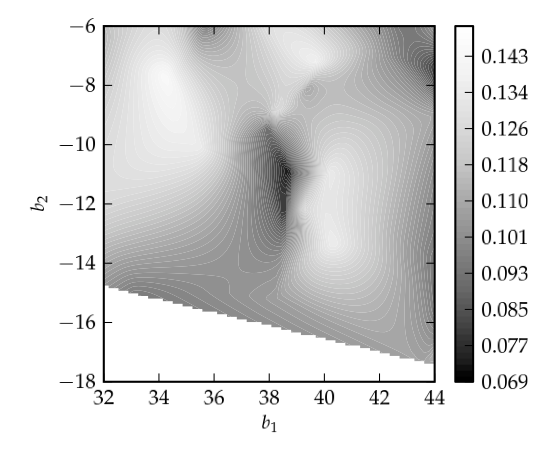
\includegraphics[height=0.5\textwidth,  clip]{figures/imrimri/b1b2_mapb1b2m1m6no.eps}
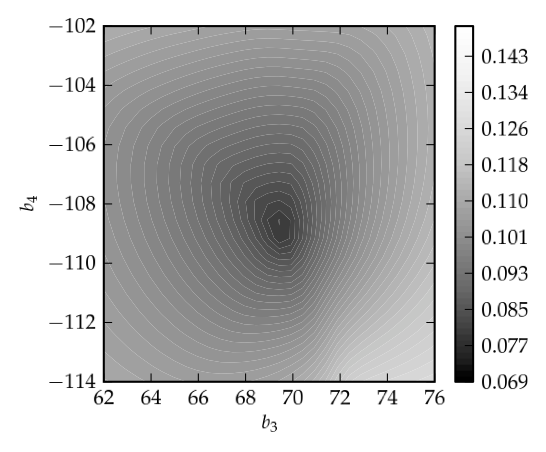
\includegraphics[height=0.5\textwidth,  clip]{figures/imrimri/b3b4_mapb3b4m1m6no.eps}
}
\centerline{
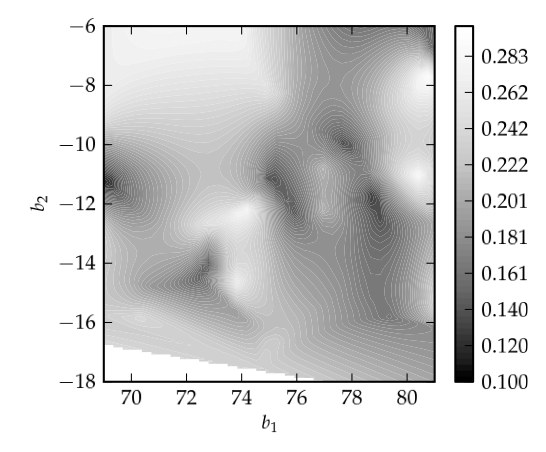
\includegraphics[height=0.5\textwidth,  clip]{figures/imrimri/b1b2_mapb1b2m1m8no.eps}
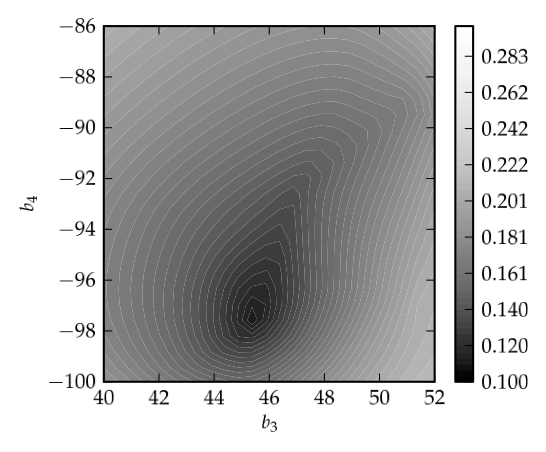
\includegraphics[height=0.5\textwidth,  clip]{figures/imrimri/b3b4_mapb3b4m1m8no.eps}
}
\caption{The (top, \, bottom) panels show the results of the optimization runs that were used to constrain the values of the \(b_i\) coefficients given in Eq.~\eqref{etacorrect}. The panels show the results for binaries of mass--ratio \(q\in [1/6,\, 1/8]\), and total mass \(M= [7M_{\odot},\,   9M_{\odot}]\). The `optimal' value for the coefficients has been chosen by ensuring that the flux prescription minimizes the phase discrepancy between the EOB model and our self-force model. The color bar shows the phase difference squared between both models, which is integrated from \(r=20M\) all the way to the light-ring.} 
\label{bimaps}
\end{figure*}

It must be emphasized that even if we only use the inspiral evolution to model binaries with mass-ratios that typically describe NSBH binaries, our self-force evolution model performs better than TaylorT4, since we can reduce the phase discrepancy between TaylorT4 and EOB at the last stable circular orbit by a factor of \((\sim40, \, \sim70)\)  for binaries with \(q=(1/6,\,1/10)\)  and total mass \(M\in (7M_{\odot} ,\, 11M_{\odot} )\) (see Figure~\ref{pn_approx}).


 \begin{figure*}%[ht]
\centerline{
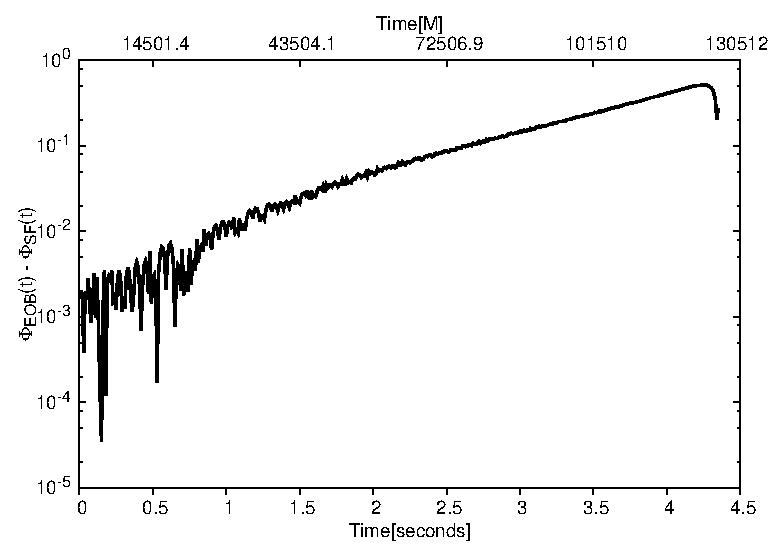
\includegraphics[height=0.4\textwidth,  clip]{figures/imrimri/phsiffeobsfm1m6.eps}
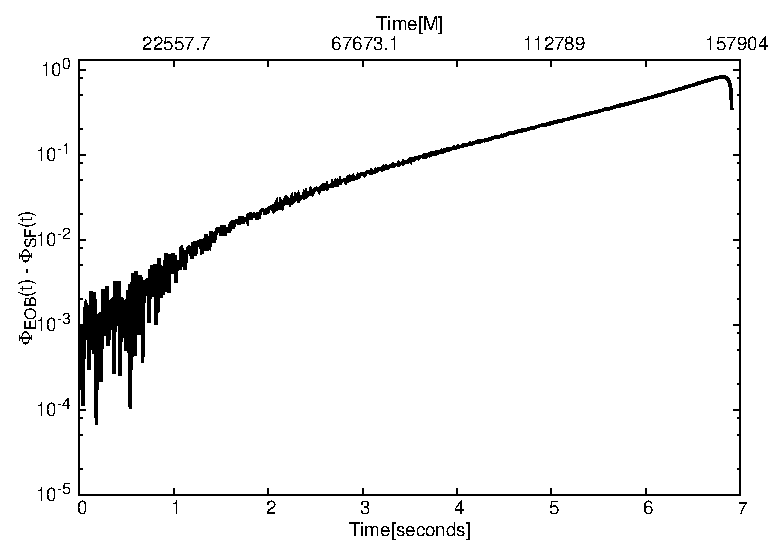
\includegraphics[height=0.4\textwidth,  clip]{figures/imrimri/phsiffeobsfm1m8.eps}
}
\centerline{
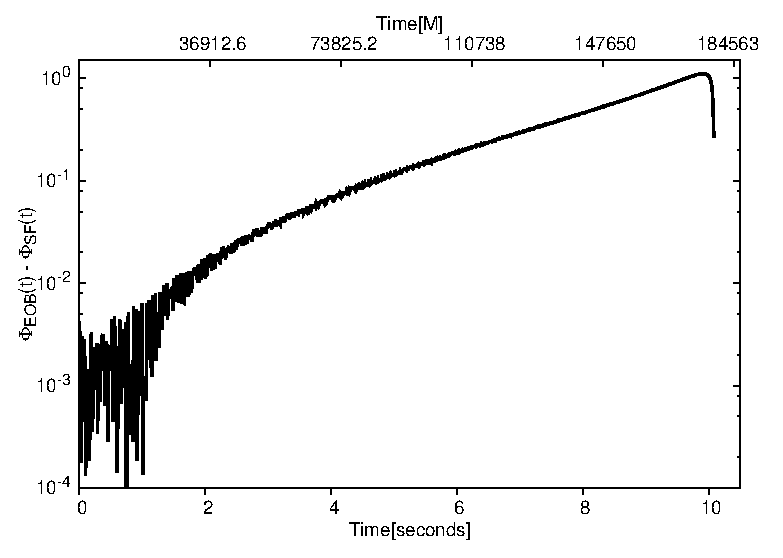
\includegraphics[height=0.4\textwidth,  clip]{figures/imrimri/phsiffeobsfm1m10.eps}
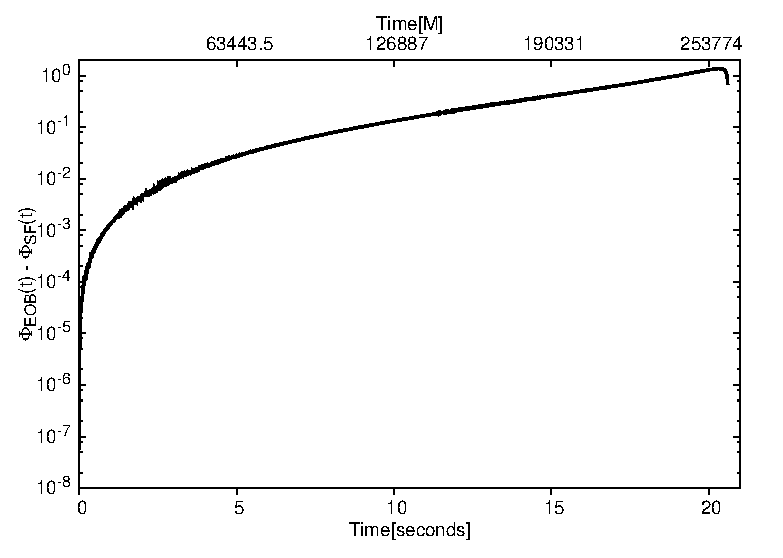
\includegraphics[height=0.4\textwidth,  clip]{figures/imrimri/phsiffeobsfm1m15.eps}
}
\caption{The panels show the orbital phase evolution of a self-force model making use of optimized PN energy flux given by Eq.~\eqref{pnfluxfit} and the phase evolution as predicted by the EOB model. The [top/bottom] panels exhibit this evolution for a compact binary with mass--ratio \(q=[(1/6,\,1/8), \,( 1/10,\,1/15)]\), and total mass \(M=[ (7M_{\odot} ,\, 9M_{\odot} ), \, ( 11M_{\odot},\, 16M_{\odot})  ]\), respectively. }
\label{PNoptimized}
\end{figure*}

Figure~\ref{PNoptimized} conveys an important message --- second order 
corrections to the radiative part of the self-force may provide a robust 
framework to describe in a single model not only events that are naturally 
described by BHPT, such as the mergers of stellar mass compact objects with
supermassive BHs in galactic nuclei~\cite{Huerta:2012, Huerta:2010, wargar,
cutler, gairles, SFB, GairL:2013}, but also events that are better described
by PN or numerical methods, in particular the coalescences of comparable
mass binaries~\cite{Huerta:2012, higherspin, Huerta:2011a, Huerta:2011b, smallbody}.

To finish this Section, we describe the construction of the gravitational
waveform from the inspiral trajectory. At leading post-Newtonian order, a 
general inspiral waveform can be written as
\begin{equation}
h(t) = -(h_{+} - i h_{\times}) = \sum_{\ell=2}^{\infty} \sum_{m=-\ell}^{l} h^{\ell m} {}_{-\!2}Y_{\ell m}(\iota,\Phi).
\label{inspwav}
\end{equation}

\noindent If only the leading-order modes \((\ell,m)=(2, \pm 2)\) and included, the inspiral waveform components  are given by 
\begin{eqnarray}
h_{+}(t)&=& \frac{4\, \mu\,  r^2\, \dot{\phi}^2 }{D}\left(\frac{1+\cos^2 \iota}{2}\right)\cos\left[2(\phi(t) + \Phi)\right],\label{inspp}\\
h_{\times}(t)&=& \frac{4\, \mu\, r^2\, \dot{\phi}^2}{D} \cos\iota \sin\left[2(\phi(t) + \Phi)\right],
\label{inspc}
\end{eqnarray}
\noindent where \(D\) is the luminosity distance to the source. Since the
orbital evolution will deviate from a circular trajectory during late 
inspiral (\(\dot{r}\neq0\)), we must consider more general orbits in which
both \(\dot{r}\) and \(\dot{r}\dot{\phi}\) are non-negligible. For such orbits,
at Newtonian order, the GW polarizations are given by~\cite{Gopakumar:2002}:
\begin{eqnarray}
\label{insppcor}
h_{+}(t)&=& \frac{2 \mu }{D}\Bigg\{ \left(1+\cos^2 \iota\right) \Bigg[ \cos\left[2(\phi(t) + \Phi)\right]\left(-\dot{r}^2 + r^2 \dot{\phi}^2 + \frac{1}{r}\right) \nonumber \\ &+& 2r\,\dot{r}\,\dot{\phi}\,\sin\left[2(\phi(t) + \Phi)\right]\Bigg] + \left(-\dot{r}^2 - r^2\dot{\phi}^2 + \frac{1}{r}\right)\sin^2 \iota\Bigg\}\,,\\
\label{inspccorrected}
h_{\times}(t)&=&\frac{4 \mu }{D}\cos\iota\Bigg\{  \sin\left[2(\phi(t) + \Phi)\right]\left(-\dot{r}^2 + r^2 \dot{\phi}^2 + \frac{1}{r}\right) \nonumber \\ &-& 2r\,\dot{r}\,\dot{\phi}\,\cos\left[2(\phi(t) + \Phi)\right]\Bigg\},
\end{eqnarray}
\noindent where \(\dot{r}\) can be computed using
\begin{displaymath}
\frac{{\mathrm{d}}r}{{\mathrm{d}}t} = -\frac{1}{u^2}\frac{{\mathrm{d}u}}{{\mathrm{d}}x}\frac{{\mathrm{d}x}}{{\mathrm{d}}t}\, .
\end{displaymath}
Having described the inspiral model, we now discuss the approach followed to
smoothly connect the late inspiral evolution onto the plunge phase. The
adiabatic prescription given by Eq.~\eqref{radev} breaks down when 
\(dE/dx\rightarrow 0\). Therefore, we need a scheme that enables us to match
the late inspiral phase onto the plunge phase. We will do this by modifying 
the ``transition'' phase, extending the method of Ori and Thorne~\cite{amos}.


\subsection{Transition and plunge phases}
\label{trans}
In this Section we describe an extension of the transition phase model introduced by Ori and Thorne~\cite{amos}. The basic idea behind this approach can be understood by studying the motion of an inspiralling object in terms of the effective potential, \(V(r, L)\), which takes the following simple form for  a Schwarzschild BH~\cite{mtw}:
\begin{equation}
V(r, L) = \left(1-\frac{2}{r} \right)\left(1+ \frac{L^2}{r^2}\right).
\label{effpot_fmrc}
\end{equation} 
\noindent Throughout the inspiral, the body moves along a nearly circular orbit, and hence the ratio of the energy flux to the angular momentum flux is given by:
\begin{equation}
 \frac{{\mathrm{d}}E}{{\mathrm{d}}\tau} = \Omega  \frac{{\mathrm{d}}L}{{\mathrm{d}}\tau}.
 \label{radII}
 \end{equation}
Near the ISCO, the energy and angular momentum of the body satisfy the following relations:
\begin{eqnarray}
\label{ener_emri}
E & \rightarrow & E_{\rm{ISCO}} + \Omega_{\rm{ISCO}}\, \xi,\\
\label{ang_emri}
L  & \rightarrow & L_{\rm{ISCO}}+  \xi.
\end{eqnarray}
\noindent Re-writing the effective potential, Eq.~\eqref{effpot_fmrc}, in terms of \(\xi = L-L_{\rm{ISCO}}\), one notices that during early inspiral, \(\xi \gg0\), the motion of the object is adiabatic, and the object sits at the minimum of the potential ---as shown in the top panel of Figure~\ref{effpotper}. However, as the object nears the ISCO, the minimum of the potential moves inward due to radiation reaction. At some point, the body's inertia prevents the body from staying at the minimum of the potential, and adiabatic inspiral breaks down~\cite{amos} --- illustrated in the bottom
panel of Figure~\ref{effpotper}.


\begin{figure*}%[ht]
% \centerline{
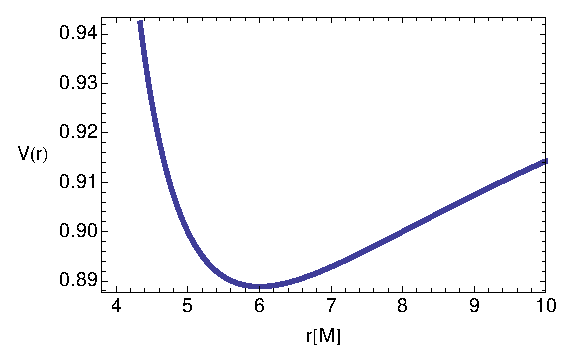
\includegraphics[height=0.6\textwidth,  clip]{figures/imrimri/effective_potential_nonpert.eps}
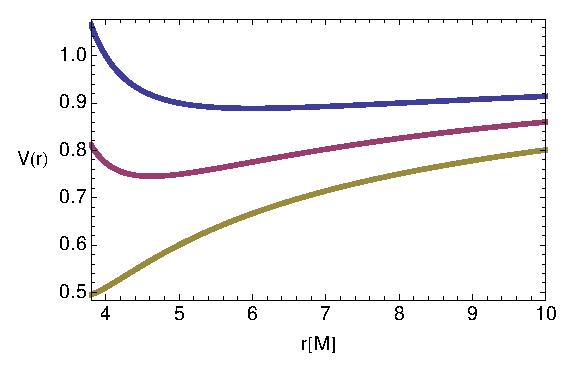
\includegraphics[height=0.6\textwidth,  clip]{figures/imrimri/effective_potential_pert.eps}
% }
\caption{Top panel: The object sits at the minimum of the effective potential, Eq.~\eqref{effpot_fmrc}, which corresponds to the case  \(\xi = L-L_{\rm{ISCO}} \gg 0\). Bottom panel. Blue (top) curve: radial geodesic motion, which corresponds to \(\xi = L-L_{\rm{ISCO}} \gg 0\);  Red (middle) curve: the object nears the ISCO and the orbit shrinks due to radiation reaction. Note that the minimum of the potential has moved inwards (\(\xi = 0.35\)). Yellow (bottom) curve:  body's inertia prevents it from staying at the minimum of the potential, and adiabatic inspiral breaks down  (\(\xi = 0\)). At this point the transition regime takes over the late inspiral evolution~\cite{amos}. Note: this plot is based on Figure 1 of~\cite{amos}.}
\label{effpotper}
\end{figure*}

\noindent The equation that governs the radial motion during the transition regime is found by linearising the equation 
\begin{equation}
\left(\frac{{\mathrm{d}}r}{{\mathrm{d}}\tau}\right)^2 = E(r)^2 - V(r,\,L),
\label{geoeom}
\end{equation}
\noindent using Eqs.~\eqref{ener_emri}, \eqref{ang_emri}, and
\begin{equation}
\label{xi_eq}
\frac{{\mathrm{d}}\xi}{{\mathrm{d}}\tau}= \kappa\, \eta, \quad {\rm{with}} \quad \kappa =\bigg[\frac{32}{5}\Omega^{7/3} \frac{\dot{{\cal{E}}}}{\sqrt{1-3u}}\bigg]_{\rm{ISCO}} \,,
\end{equation}
\noindent where \(\dot{{\cal{E}}}\) is the general relativistic correction to the Newtonian, quadrupole-moment formula~\cite{ori}. We now extend these Eqs. by including finite mass-ratio corrections. Eq.~\eqref{geoeom} can be replaced by 
\begin{equation}
\frac{{\mathrm{d}}x}{{\mathrm{d}}t}= \frac{u^2(1-2u)}{E(x) }\left(\frac{{\mathrm{d}}u}{{\mathrm{d}}x}\right)^{-1} \bigg[E(x)^2 - V\left(u(x),L(x)\right)\bigg]^{1/2},
\label{eomfmrc}
\end{equation}
 \noindent where we have used
 \begin{equation}
 \frac{{\mathrm{d}}\tau}{{\mathrm{d}}t}= \frac{1-2\,u(x)}{E(x)}\,,
 \label{tfact}
 \end{equation}
\noindent and the expressions for the energy and angular momentum are given by Eqs.~\eqref{enofxeq}, \eqref{lzofxeq}. In order to linearize Eq.~\eqref{eomfmrc} we replace $E(x)$ and $L(x)$ by Eqs~\eqref{ener_emri} and \eqref{ang_emri} respectively.

\begin{figure*}%[ht]
% \centerline{
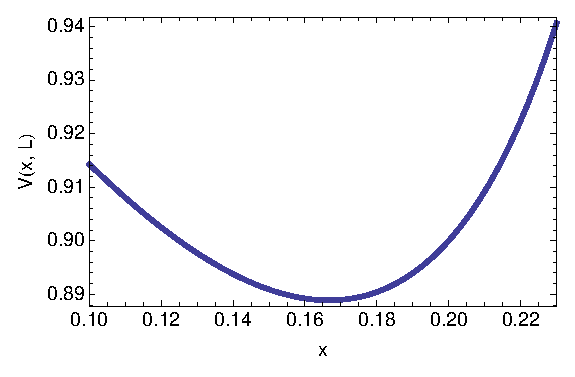
\includegraphics[height=0.6\textwidth,  clip]{figures/imrimri/pot_eta_limit.eps}
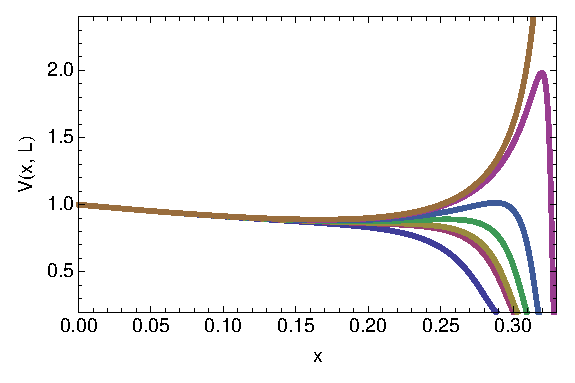
\includegraphics[height=0.6\textwidth,  clip]{figures/imrimri/mod_eff_pot.eps}
% }
\caption{The top panel shows the effective potential for a Schwarzschild BH 
{\it without} including finite mass--ratio corrections. Note that the minimum
of the potential takes place at the ISCO, which can be determined using 
Eq.~\eqref{xisco_eq}.  The bottom panel exhibits the influence of finite 
mass-ratio corrections on the effective potential used to modify Ori and 
Thorne transition regime~\cite{amos}. The curves represent  binaries 
(top to bottom) with mass-ratios  
\(q \in [0,\, 1/100, \,1/20, \,1/10, \,1/6, \,1/5, \,1 ]\).}
\label{eff_pot_fig}
\end{figure*}

As discussed in~\cite{amos}, since these equations use the \(\eta\)-corrected values for \(E(x_{\rm{ISCO}} )\), \(L(x_{\rm{ISCO}}) \) and \( \Omega_{\rm{ISCO}}\), then they remain valid even for finite mass-ratio \(\eta\)~\cite{amos}. In Figure~\ref{eff_pot_fig} we show the effect that these finite mass-ratio \(\eta\) corrections have on the effective potential \(V(x, L(x))\). We determine the point at which the transition regime starts by carrying out a stability analysis near the ISCO using \({\mathrm{d}} E/ {\mathrm{d}} x\). As shown in Figure~\ref{dedx}, the ISCO is determined by the relation \({\mathrm{d}} E/{\mathrm{d}} x =0\). We have found that the relation 
\begin{equation}
\left(\frac{{\mathrm{d}}E}{{\mathrm{d}}x}\right)\Bigg |_{\rm{transition}} = -0.054 + \frac{1.757\times10^{-4}}{\eta}\,,
\label{transition_point}
\end{equation}
\noindent provides a robust criterion to mark the start of the transition regime for binaries with mass-ratios \(1/100<q<1/6\).  


In~\cite{ori}, the authors only kept terms linear in \(\xi\), but we have explored which higher order terms had a noticeable impact on the evolution by examining their impact on the length  and phasing of the waveform. We found that terms  \(\propto \xi\) and \( \propto (u- u_{\rm{ISCO}})\xi\) were important, but corrections at order \({\cal{O}}(\xi^2)\) could be ignored even for comparable mass-ratio systems.

We model the evolution of the orbital frequency during the transition regime and thereafter in a  different manner to that proposed by Ori and Thorne~\cite{amos}. In order to ensure that the late-time evolution of the orbital frequency of our self-force model is as close as possible to the orbital evolution extracted from numerical relativity simulations, we incorporate the late-time frequency evolution that was derived by Baker et al~\cite{Baker:2008} in their implicit rotating source (IRS) model, namely:
\begin{equation}
\frac{d \phi}{d \mathrm{t} }  = \Omega_{\rm{i}}+ \left(\Omega_{\rm{f}}\  -\Omega_{\rm{i}}\right)\left(\frac{1 + \tanh( \ln\sqrt\varkappa + (t-t_0)/b)}{2}\right)^{\varkappa}\, ,
\label{late_frequency}
\end{equation}
\noindent where \( \Omega_{\rm{i}}\) is the value of the orbital frequency when the transition regime begins, and  \( \Omega_{\rm{f}}\) is the value of the frequency at the light ring, which corresponds to \(\omega_{\rm{\ell m n}}/m\), where \(\omega_{\rm{\ell m n}}\) is the fundamental quasi-normal ringing frequency \((n=0)\) for the fundamental mode \((\ell, m) = (2,2)\) of the post-merger black hole (see Eq.~\eqref{finspin} below).  The constant mass-dependent coefficient \(t_0\) is computed by ensuring that \(d\Omega/dt\) peaks at a time \(t=t_0\). The parameter \(\varkappa\) is computed by enforcing continuity between the first order time derivative of the orbital frequency as predicted by the self-force evolution ---Eq.~\eqref{new_phase}--- and that given by the first order time derivative of Eq.~\eqref{late_frequency}.

% At the end of the plunge phase, we match the plunge waveforms, which are generated using Eqs.~\eqref{insppcor}, \eqref{inspccorrected}, onto the \(l=m=2\), \(n=0\) ringdown mode since this dominates the ringdown radiation. In the following Section we will describe in detail the procedure followed to attach the ringdowm waveform. 

After the transition regime, the plunge phase equations of motion are:  the second order time  derivative of Eq.~\eqref{eomfmrc} which gives the radial evolution, and Eq.~\eqref{late_frequency} which describes the orbital frequency evolution. We determine the point at which to attach the plunge phase by integrating  Eq.~\eqref{eomfmrc} backwards in time, and finding the point at which the transition and plunge equations of motion smoothly match. 


\begin{figure*}[ht]
\centerline{
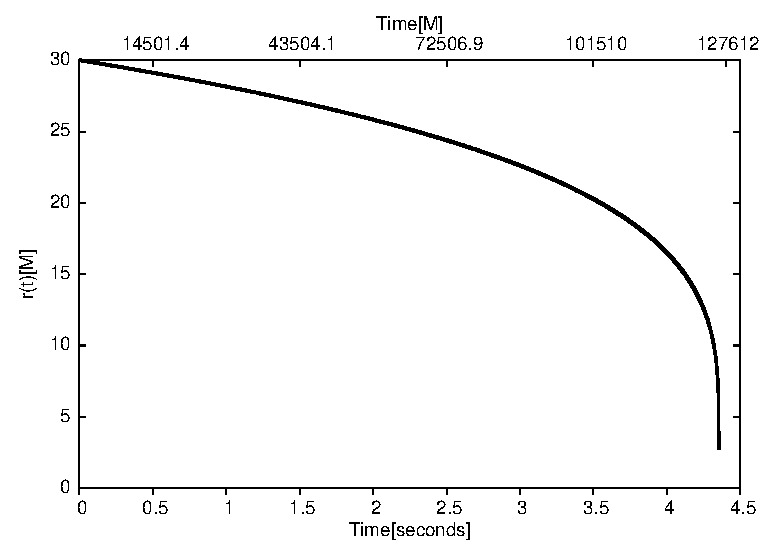
\includegraphics[height=0.4\textwidth,  clip]{figures/imrimri/rvstm1m6.eps}
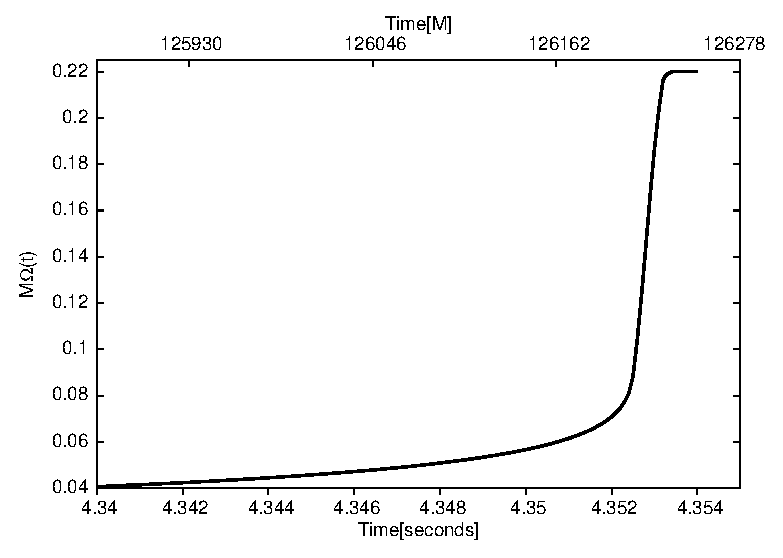
\includegraphics[height=0.4\textwidth,  clip]{figures/imrimri/xvsMOmegam1m6.eps}
}
\centerline{
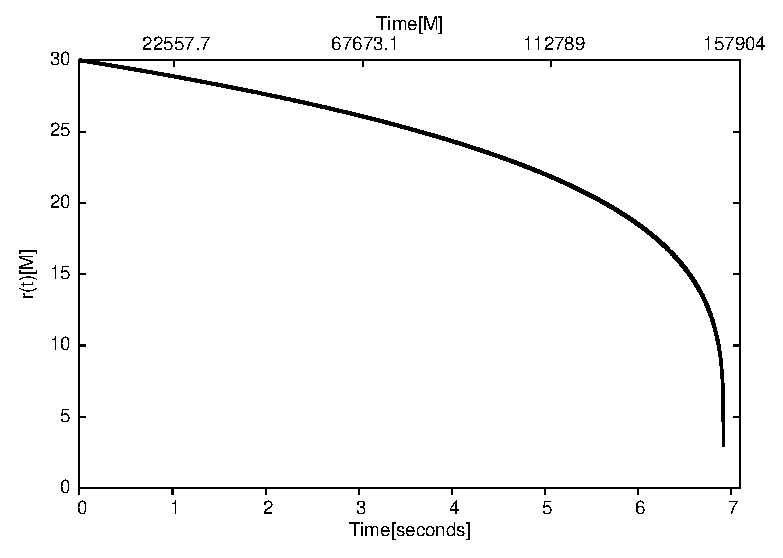
\includegraphics[height=0.4\textwidth,  clip]{figures/imrimri/rvstm1m8.eps}
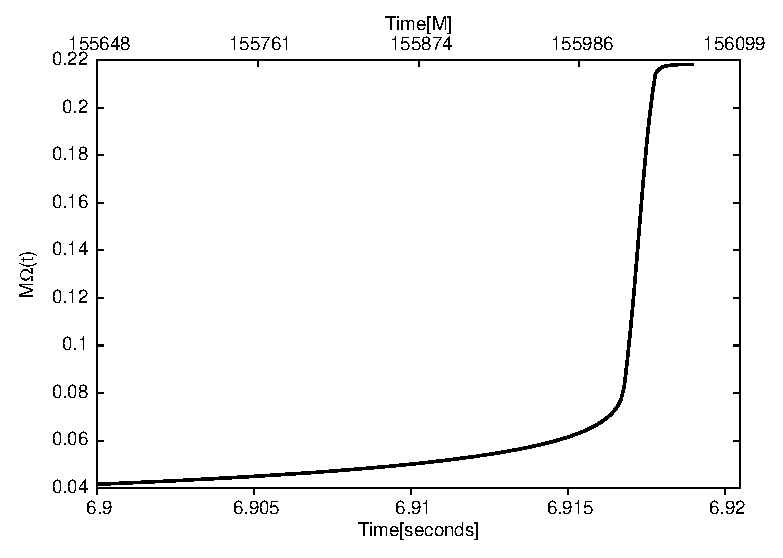
\includegraphics[height=0.4\textwidth,  clip]{figures/imrimri/xvsMOmegam1m8.eps}
}
\caption{(Top, bottom) panels: the left panel shows the inspiral, transition and plunge radial evolution for a BH binary of mass-ratio \(q=(1/6,\,1/8)\) --- and total mass \(M\in (7M_{\odot} ,\, 9M_{\odot} )\) --- using the coordinate transformation given by Eq.~\eqref{rofx}. The right panel shows the orbital frequency \(M\Omega\) from late inspiral all the way to the light ring. The evolution starts from an initial radial value \(r=30M\).}
\label{IP}
\end{figure*}

\begin{figure*}[ht]
\centerline{
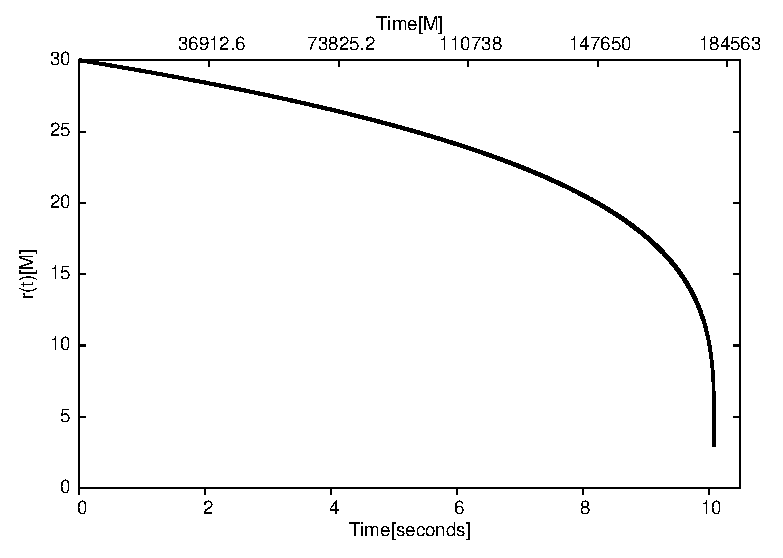
\includegraphics[height=0.4\textwidth,  clip]{figures/imrimri/rvstm1m10.eps}
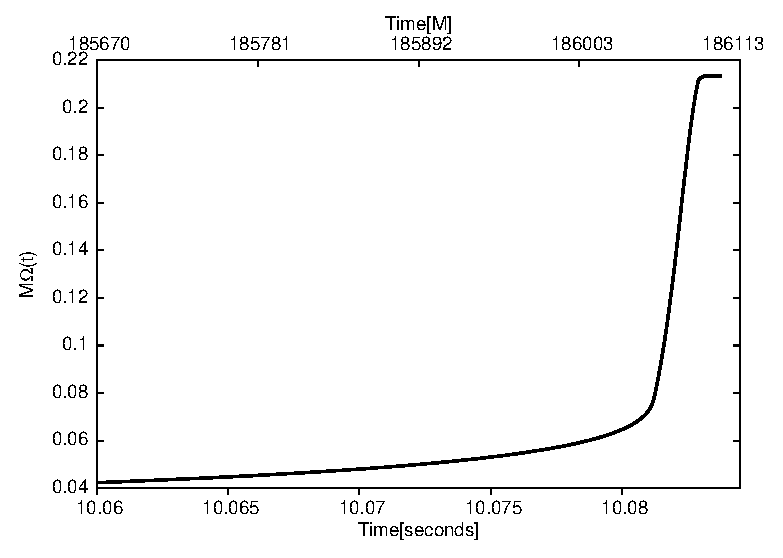
\includegraphics[height=0.4\textwidth,  clip]{figures/imrimri/xvsMOmegam1m10.eps}
}
\centerline{
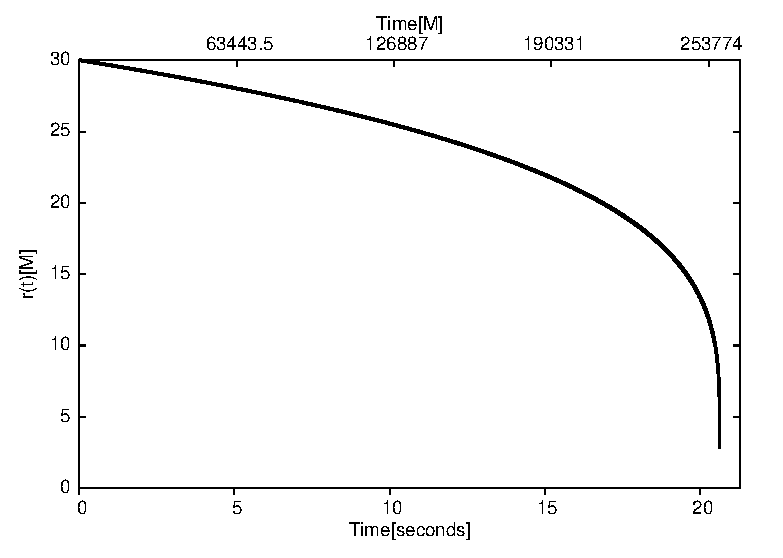
\includegraphics[height=0.4\textwidth,  clip]{figures/imrimri/rvstm1m15.eps}
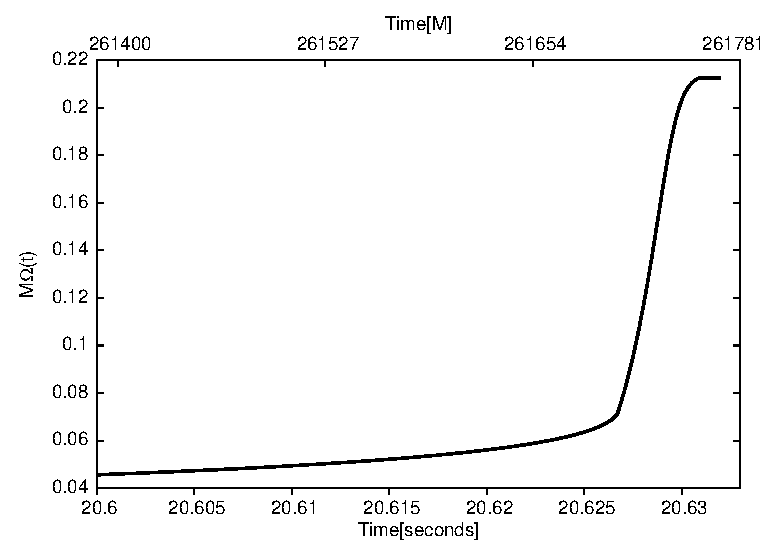
\includegraphics[height=0.4\textwidth,  clip]{figures/imrimri/xvsMOmegam1m15.eps}
}
\caption{As in Figure~\ref{IP}, but with the (top, bottom) panels showing the radial and orbital frequency evolution for binaries with mass--ratios \(q=(1/10,\,1/15)\), and total mass \(M\in( 11M_{\odot},\, 16M_{\odot})  \), respectively.  As before, the evolution starts from an initial radial value \(r=30M\).}
\label{IPI}
\end{figure*}


In Figures~\ref{IP} and \ref{IPI} we show the evolution obtained by combining Ori and Thorne's~\cite{amos} transition approach for the radial motion with the frequency evolution proposed by Baker et al~\cite{Baker:2008}.   In all the cases shown in Figures~\ref{IP} and \ref{IPI}, the orbital frequency peaks and saturates at the value given by \(\omega_{\ell m n}/m\). This can be understood if we analyze the asymptotic behavior of Eq.~\eqref{late_frequency} near the light-ring, i.e.,
\begin{equation}
\frac{d \phi}{d \mathrm{t} }  \approx \Omega_{\rm{f}} -  \left(\Omega_{\rm{f}}\  -\Omega_{\rm{i}}\right)e^{ -2(t - t_0)/b}.
\label{frequency_LR}
\end{equation}
Recasting Eq.~\eqref{late_frequency} in this form, enables us to identify the
constant coefficient \(b\) with the e-folding rate for the decay of the 
fundamental quasinormal mode (QNM). Using the IRS model for frequency evolution
therefore allows for a smooth transition from late inspiral to the plunge phase.

% As discussed previously,  
% Eq.~\eqref{late_frequency} predicts the expected orbital evolution during late
% inspiral and onward. 
% 
% To provide a unified description from late inspiral through to ringdown, we have decided to adopt the IRS approach, since this framework allows us to smoothly transition from late inspiral  onto the plunge phase, and finally describe the ringdown waveform as a natural consequence of the IRS strain-rate amplitude decay relation \(A^2(t) \propto \Omega \dot{\Omega}\)~\cite{Baker:2008}. In other words, since Eq.~\eqref{frequency_LR} has the correct behavior near the light-ring as predicted by BHPT, the IRS model provides a natural framework to attach the ringdowm waveform at the end of the plunge phase. We will discuss this feature in further detail in the following Section.

\subsection{Ringdown Waveform}
\label{RDwav}

 Numerical relativity simulations have shown that coalescing binary BHs in 
 general relativity lead to the formation of a distorted rotating remnant,
 which radiates GWs while it settles down to a stationary Kerr
 BH~\cite{Berti:2006, Berti:2006b}. The GWs emitted during this intermediate
 phase resemble a ringing bell. Hence, this type of radiation is commonly 
 known in the literature as ringdown radiation, and consists of a superposition
 of QNMs --- first discovered in numerical studies of the scattering of GWs
 in the Schwarzschild spacetime by Vishveshwara~\cite{Vish:1970}.   QNMs are
 damped oscillations whose frequencies are uniquely determined by the mass 
 and spin of the post-merger Kerr BH.  The frequency \(\hat \omega\) of each 
 QNM has two components: the real part represents the oscillation frequency, 
 and the imaginary part corresponds to the inverse of the damping time:
 \begin{equation}
 \hat \omega = \omega_{\ell m n} - i/\tau_{\ell m n}.
 \label{omega_QNM}
 \end{equation}
\noindent As discussed above, the observables 
\(\omega_{\ell m n}, \, \tau_{\ell m n}\) are uniquely determined by the final
mass, \(M_{\rm{f}}\), and final spin, \(q_{\rm{f}}\), of the post-merger Kerr BH.
The mass of the post-merger BH  \(M_{\rm{f}}\) is modeled using the 
phenomenological fit proposed in~\cite{Barausse:2012},
\begin{equation}
\frac{M_{\rm{f}}}{M} = 1- \left(1-\frac{2\sqrt{2}}{3}\right)\eta - 0.543763\, \eta^2.
\label{finalmass}
\end{equation}
% 
This expression reproduces the expected result in the test-particle 
limit, and also reproduces results from currently available NR
simulations~\cite{Barausse:2012,spif}. We determine the final spin of the 
BH remnant  \(q_{\rm{f}}\) using the fit proposed in~\cite{Bounanno:2007}:
\begin{equation}
q_{\rm{f}} =    \sqrt{12}\, \eta + s_1\,\eta^2 + s_2\,\eta^3,
\label{finspin}
\end{equation}
with
\begin{gather}
s_1=-3.454\pm0.132, \qquad  s_1=2.353\pm0.548.
\label{spin_coeff}
\end{gather}
\noindent This prescription is consistent with the numerical relativity
simulations described in~\cite{Bounanno:2007,spif}, and reproduces test-mass
limit predictions. This compact formula is also consistent with the  
prescriptions introduced in~\cite{Barus:2009,Rezzolla:2008}. The largest
discrepancy between Eq.~\eqref{finspin} and those derived in~\cite{Barus:2009,
Rezzolla:2008}  is \(\lesssim2.5\%\) for binaries with \(q\lesssim1/6\). 
The ringdown waveform is given by~\cite{Berti:2006b, Baker:2008}
\begin{eqnarray}
h(t)&=& -\left(h_{+} - i h_{\times}\right) = \frac{ M_{\rm{f}} }{D} \sum_{\ell m n} {\cal{A}}_{\ell m n}\,e^{-i \left(  \omega_{\ell m n}\, t  + \phi_{\ell m n} \right)} \, e^{-t/\tau_{\ell m n} }\,, 
\label{waverd}
\end{eqnarray}
where \(  {\cal{A}}_{\ell m n} \) and \( \phi_{\ell m n}\) are constants to be determined by smoothly matching the plunge waveform onto the subsequent ringdown. The ringdown portion of the self-force waveform model constructed in this chapter includes the mode \(\ell=m=2\) and the tones \(n=0,\, 1, \, 2\). The approach we follow to attach the leading mode and overtones is the following: 

\begin{itemize}
\item In order to ensure continuity between the plunge and ringdown waveforms, we use the end of the plunge waveform --- Eqs.~\eqref{insppcor}, \eqref{inspccorrected} --- to construct an interpolation function \(F(t)\). The interpolation method used to construct \(F(t)\) is a cubic spline.
\item We match the plunge waveform onto the leading mode  \(\ell=m=2\), \(n=0\)  of the ringdown waveform, Eq.~\eqref{waverd}, at the point where the amplitude of the plunge waveform peaks, \(t_{\rm{max}}\). Attaching the mode requires \(F(t=t_{\rm{max}})\) and \(F'(t=t_{\rm{max}})\) which are computed from the interpolation function. These conditions fix two constants per polarisation.
\item To attach the first overtone,  \(\ell=m=2,\, n=1\),   we insert into Eq.~\eqref{waverd} the constants determined by attaching the leading mode as seeds to compute the amplitude and phase coefficients for the first overtone by enforcing continuity at  \(t_{\rm{max}} + dt\).
\item Finally, we insert into  Eq.~\eqref{waverd} the value of the amplitude and phase coefficients previously determined for the leading mode and first overtone, and determine the four remaining constants by enforcing continuity at \(t_{\rm{max}} + 2\,dt\).
\end{itemize} 


Having described the methodology followed to construct complete waveforms for comparable and intermediate mass-ratio systems, we finish this Section by putting together all these various pieces to construct sample waveforms for a few systems with mass-ratio \(q\in[1/6,\,1/8,\, 1/10,\, 1/15]\), and total mass  \(M\in( 7M_{\odot},\, 9M_{\odot},\, 11M_{\odot},\, 16M_{\odot}) \) in Figure~\ref{Completewavs}. 

\begin{figure*}[ht]
\centerline{
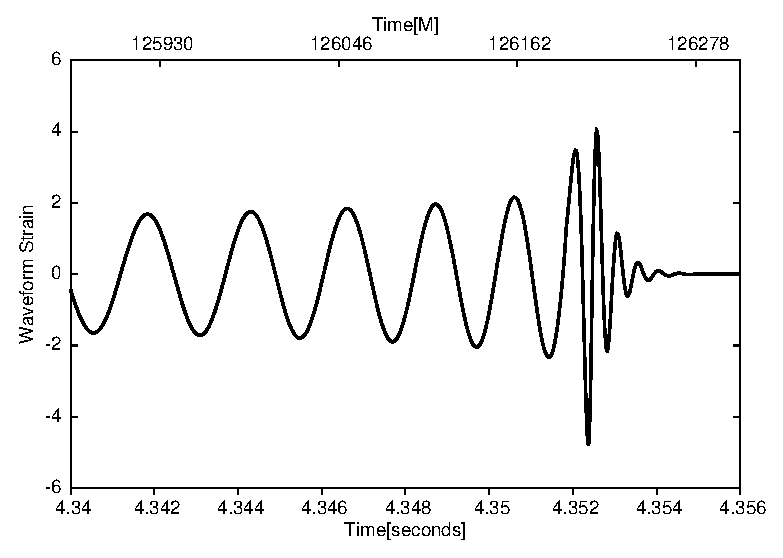
\includegraphics[height=0.4\textwidth,  clip]{figures/imrimri/wavem1m6complete.eps}
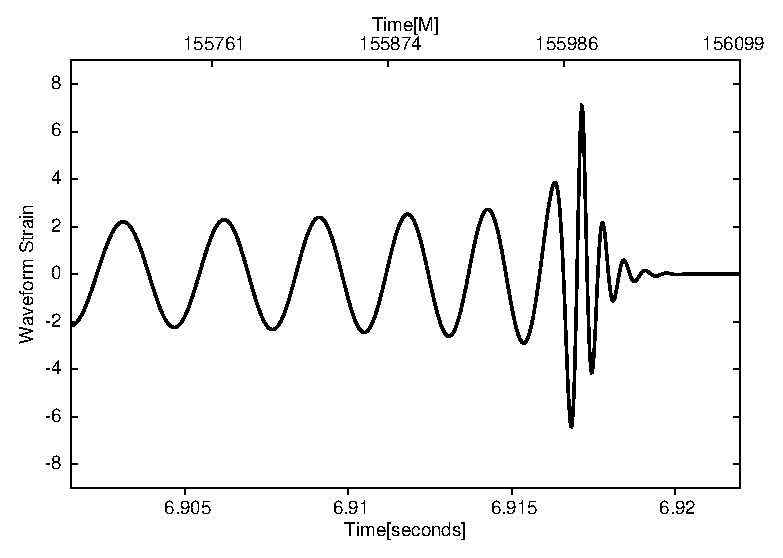
\includegraphics[height=0.4\textwidth,  clip]{figures/imrimri/wavem1m8complete.eps}
}
\centerline{
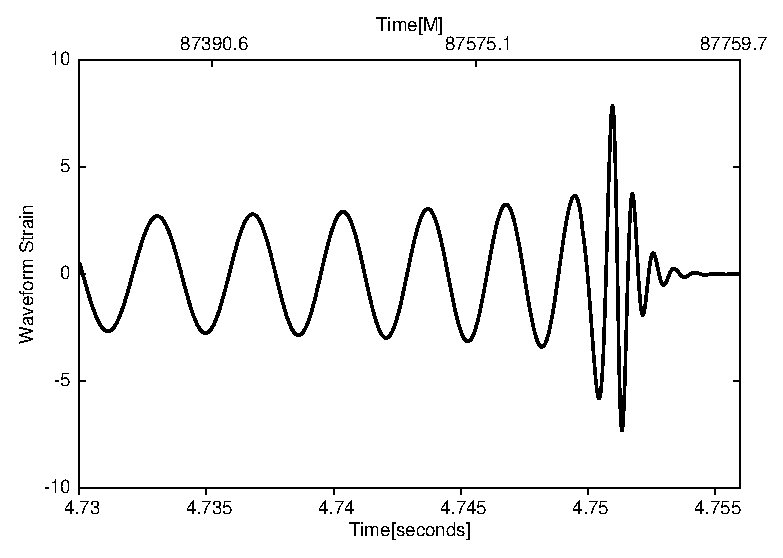
\includegraphics[height=0.4\textwidth,  clip]{figures/imrimri/wavem1m10complete.eps}
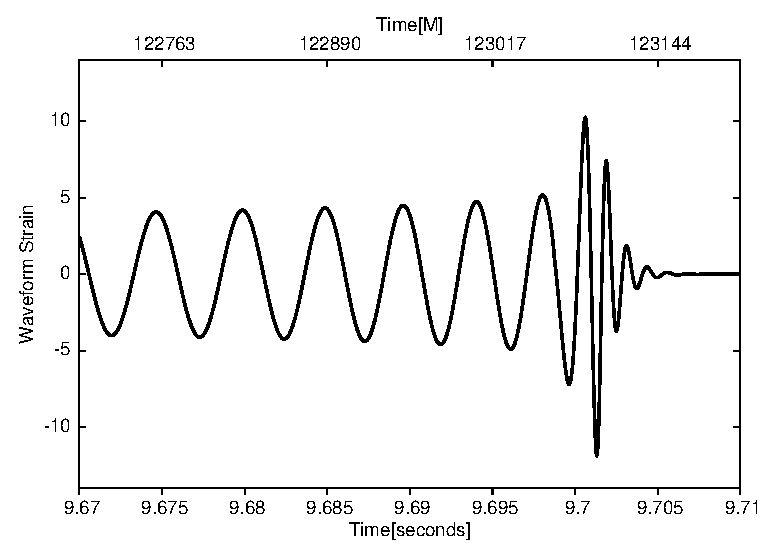
\includegraphics[height=0.4\textwidth,  clip]{figures/imrimri/wavem1m15complete.eps}
}
\caption{The panels show sample waveforms from inspiral to ringdown for systems with mass-ratios \(q\in[1/6,\,1/8]\) ---and total mass  \(M\in( 7M_{\odot},\, 9M_{\odot}) \)--- (top panels---from left to right) and \(q\in[1/10,\, 1/15]\)  ---and total mass  \(M\in( 11M_{\odot},\, 16M_{\odot}) \)--- (bottom panels ---from left to right). The inspiral evolution for the [top,\, bottom] panels starts from  \(r=[30M,\, 25M]\). }
\label{Completewavs}
\end{figure*}

% \subsection{ Ringdown waveform construction in the context of an Implicit Rotating Source}
% 
% Having described the ringdown waveform construction as a sum of quasinormal modes, we finish this Section  by exhibiting the power of the IRS model to describe the ringdown evolution. In the IRS model, the strain-rate amplitude decay is given by~\cite{Baker:2008}:
% \begin{equation}
% A^2(t) = 16\,\pi\, \dot{E} \approx 16\,\pi\,\xi\,\Omega\,\dot{\Omega}\,.
% \label{amp_rate}
% \end{equation}
% \noindent Using~Eq.~\eqref{frequency_LR}, in the limit \(\Omega \rightarrow \Omega_{\rm{f}}\), the amplitude decay is given by
% \begin{equation}
% A_0^2\,e^{-2t/\tau} \approx \frac{32\, \pi\,\xi\, \Omega_{\rm{f}}}{b}\left(\Omega_{\rm{f}} - \Omega_{\rm{i}}\right) e^{-2(t-t_0)/\tau}\,.
% \label{rateamp}
% \end{equation}
% \noindent Hence, the late-time amplitude in the IRS model is given by
% \begin{equation}
% A^2_{\ell m}  \approx 16\,\pi\,\xi_{\ell m}\,\omega_{\ell m}\,\dot{\omega}_{\ell m}\,,
% \label{amp_rate_IRS}
% \end{equation}
% \noindent where the value of \(\xi_{\ell m}\) is set by ensuring amplitude continuity at the light-ring. In Figure~\ref{QNMvsIRS} we explicitly show the equivalence of the ringdown waveform construction  both in the IRS approach and using the sum of QNMs utilized in the previous Section. This analysis shows that the IRS is a powerful tool  to model the late time portions of the waveforms in a unified way. 
% 
% 
% \begin{figure*}[ht]
% \centerline{
% 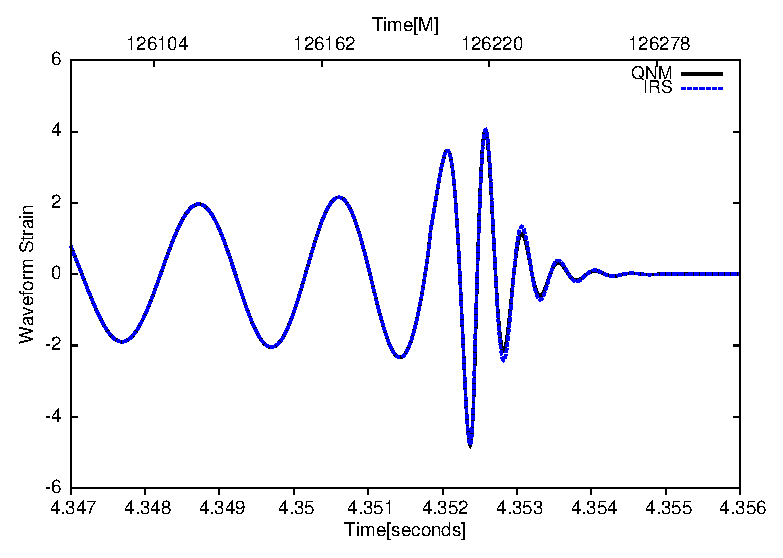
\includegraphics[height=0.35\textwidth,  clip]{figures/imrimri/QNMvsIRSm1m6.eps}
% 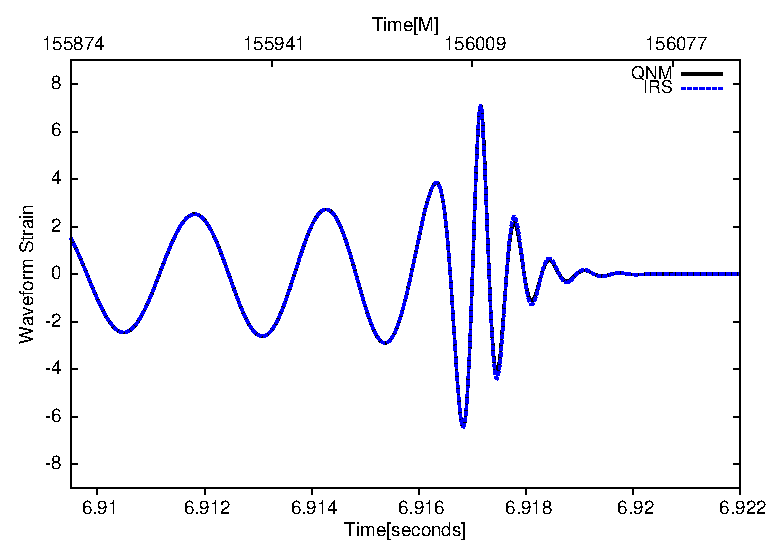
\includegraphics[height=0.35\textwidth,  clip]{figures/imrimri/QNMvsIRSm1m8.eps}
% }
% \centerline{
% 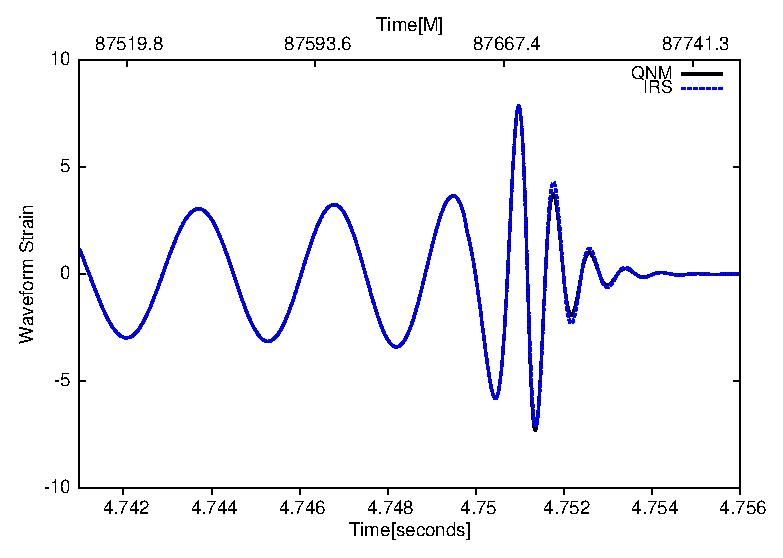
\includegraphics[height=0.35\textwidth,  clip]{figures/imrimri/QNMvsIRSm1m10.eps}
% 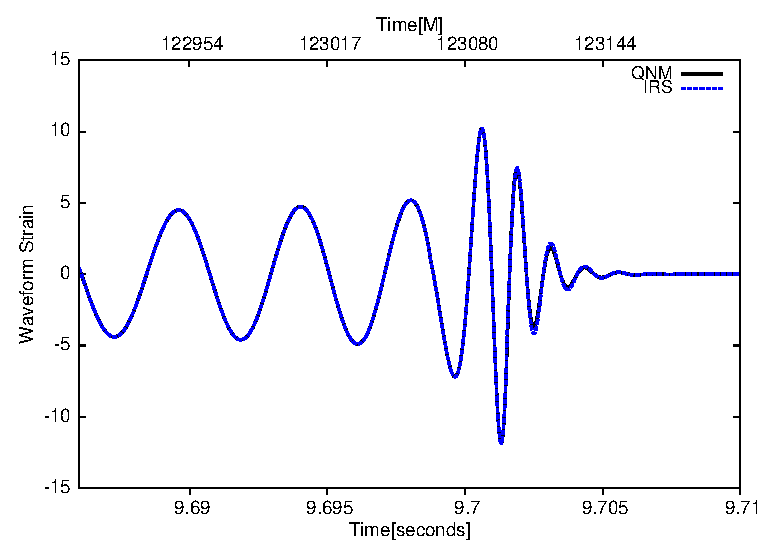
\includegraphics[height=0.35\textwidth,  clip]{figures/imrimri/QNMvsIRSm1m15.eps}
% }
% \caption{The panels show sample the late-time evolution of waveforms whose ringdown phase is modeled using the implicit rotating source (IRS) model and a sum of quasinormal modes (QNMs). The systems shown correspond to binaries with mass-ratios \(q\in[1/6,\,1/8]\) ---and total mass  \(M\in( 7M_{\odot},\, 9M_{\odot}) \)--- (top panels---from left to right) and \(q\in[1/10,\, 1/15]\)  ---and total mass  \(M\in( 11M_{\odot},\, 16M_{\odot}) \)--- (bottom panels ---from left to right). The inspiral evolution for the [top,\, bottom] panels starts from  \(r=[30M,\, 25M]\). }
% \label{QNMvsIRS}
% \end{figure*}

\subsection{Summary}
In this Section we briefly summarize the key ingredients that were used to develop the waveform model described in this chapter:
\begin{itemize}
\item{Inspiral evolution}
\begin{itemize}
\item The building blocks of the inspiral evolution are the expressions for the energy, \(E\), and angular momentum, \(L\), --- Eqs.~\eqref{enofxeq} and~\eqref{lzofxeq} --- that include gravitational self-force corrections and are valid over the domain \(0<x<\frac{1}{3}\)~\cite{Akcay:2012}.
\item The orbital frequency is modeled using Eq.~\eqref{new_phase}. This prescription encapsulates gravitational self-force corrections that render a better phase evolution when calibrated against EOB.
\item The inspiral trajectory is modeled using the simple prescription~\eqref{radev}. This scheme is no longer valid near ISCO, where \(dE/dx =0\) for binaries with \(q\leq 6\).
\item We construct the inspiral waveform using Eqs.~\eqref{insppcor}, \eqref{inspccorrected}.
\end{itemize}
\end{itemize}
% 
In order to improve the radiative evolution, we derive the second-order
corrections to the flux of energy. This was necessary in order to construct 
a waveform model that is internally consistent, i..e, since the orbital elements
include first-order conservative corrections, then radiative corrections should
enter the flux at second order. We calibrate these corrections by enforcing a
close agreement between our self-force model and EOB. We show that our model
can reproduce the orbital phase evolution predicted by EOB within the numerical
error of the NR simulations used to calibrate the EOB model itself.
% 

When the inspiralling object nears the ISCO, we need to invoke the `transition scheme' introduced by Ori and Thorne~\cite{amos}, which enables us to smoothly attach the late inspiral evolution onto the plunge phase. 

\begin{itemize}
\item{Transition phase}
\begin{itemize}
\item The transition regime starts at a point when \( \mathrm{d} E/ \mathrm{d}  x\) satisfies Eq.~\eqref{transition_point}.
\item The equations of motion that govern the transition phase are~\eqref{ener_emri}, ~\eqref{ang_emri}. These relations are valid, since the motion near the ISCO is nearly-circular. 
\item Using Eqs.~\eqref{ener_emri}, ~\eqref{ang_emri}, we linearize the second order time derivative of Eq.~\eqref{eomfmrc}.
\item In order to reproduce the orbital phase evolution predicted by numerical simulations from the ISCO to the light-ring, we modify the original transition phase by smoothly matching the inspiral orbital phase evolution, Eq.~\eqref{new_phase}, onto the IRS model, Eq.~\eqref{late_frequency} at the start of the transition phase. 
\end{itemize}
\end{itemize}

\begin{itemize}
\item{Plunge phase}
\begin{itemize}
\item The equations of motion that govern the plunge phase are given by the second order time derivative of Eq.~\eqref{eomfmrc}, and Eq.~\eqref{late_frequency}.
\item We integrate these relations backwards in time to find the point at which both the transition and plunge equations of motion smoothly match. The transition phase ends at this point.
\item Near the light-ring Eq.~\eqref{late_frequency} has the behavior predicted by BHPT, which enables us to smoothly match the plunge phase onto the ringdown. %Put in different words, we don't need to interpolate the orbital frequency evolution to attain the expected value of the orbital frequency at the light-ring. 
\item Both the transition and plunge waveforms are constructed using Eqs.~\eqref{insppcor} and \eqref{inspccorrected}.
\end{itemize}
\end{itemize}


\begin{itemize}
\item{Ringdown phase}
\begin{itemize}
\item The ringdown waveform is constructed using Eq.~\eqref{waverd}.
\item We use the plunge waveform to construct an interpolation function \(F(t)\), and then use this function to attach the leading mode \(\ell=m=2,\, n=0\) at the point where the amplitude of the plunge waveform peaks, \(t_{\rm{max}}\). We enforce continuity by ensuring that \(F( t_{\rm{max}}) = h^{n=0}_{\rm{RD}}\) and  \(F'( t_{\rm{max}}) = h'^{n=0}_{\rm{RD}}\).
\item We include the first and second overtone \(n=1,\, n=2\) in the ringdown waveform.
% \item  Using the IRS model, we have shown that having knowledge of the time evolution of the orbital frequency provides sufficient information to construct the amplitude decay during ringdowm. Hence, we can construct an alternative ringdowm waveform using only Eq.~\eqref{amp_rate_IRS}, and ensuring smooth continuity with the plunge waveform. 
% \item Finally, we have explicitly shown that the implicit rotating source approach provides a natural transition from late-time radiation to ringdown that is equivalent to ringdown waveform modeling based on a sum of QNMs.
\end{itemize}
\end{itemize}

Throughout the chapter we have emphasized the fact that our model provides a more reliable framework to model binaries whose components are non-spinning, and with mass-ratios \(q\leq 1/6\), as compared to available PN approximants. It is worth emphasizing that our model is also computationally inexpensive. All the waveforms we generated to constrain the higher-order \(\eta\) corrections in the energy flux ---Eq.~\eqref{etacorrect_new}--- can be generated in fractions of a second. A direct comparison between our code and EOB shows that, averaged over 500 realizations, our code is \(\sim20\%\) faster than the optimized version of the EOB code currently available in the LIGO Algorithms Library. It should be emphasized, though, that our code at present has not been optimized, and hence, compared to EOB our model is expected to further reduce the cost of waveform generation, making it relatively more viable for parameter estimation efforts. This is a key feature in our model that enabled 
us to sample a wide region of parameter space to constrain the \(B_i\) coefficients in Eq.~\eqref{etacorrect_new}. 
% Furthermore, these self-forced waveforms do not need to be highly sampled near the light-ring, hence decreasing the speed with which they can be generated, because the prescription we have used to model the late-time orbital frequency evolution provides the correct evolution near the light-ring. This particular feature also enables us to match the plunge waveform onto its ringdown counterpart without having to interpolate the orbital frequency evolution using a phenomenological approach.
Our model is internally consistent and the only phenomenology invoked during its construction is related to currently unknown physics, i.e., higher order radiative corrections to the energy flux. Once these corrections are formally derived in the near future, the flexibility of our model will enable us to replace the radiative corrections that we have currently computed by numerical optimization.  At that stage, we 
will be able to describe in a single unified model the dynamical evolution of binaries whose mass-ratios range from the extreme to the comparable regime. 
%\clearpage 

\section{Conclusions}
\label{conclu}

In this chapter we have developed a self-force waveform model that captures the
inspiral, merger and ringdown phases for binaries with mass-ratios 
\(q\leq 1/6\). This work suggests that a model which incorporates first-order
conservative self-force corrections in the orbital elements, and second-order
radiative corrections in the dissipative piece of the self-force, may suffice 
to describe in a unified manner the coalescence of binaries with mass-ratios 
that range from the comparable to the extreme. Using the available conservative 
self-force corrections~\cite{Akcay:2012}, we also found that binaries with
mass-ratios \(q\gtrsim1/6\) do not have an ISCO. For systems with \(q\leq1/6\),
we have derived a simple relation that provides the location of the ISCO in 
terms of the symmetric mass-ratio (see Eq.~\eqref{xisco_eq}). To describe the 
inspiral evolution, we obtain second-order corrections to the energy flux by 
minimizing the phase discrepancy between our self-force model and the EOB model~\cite{BuonannoEOBv2Main, Damour:2013} for a variety of mass-ratios. 
We show that our model reproduces the phase evolution of the EOB model within
the accuracy of available numerical simulations for a variety of mass-ratios. 

This chapter also presents an extension of the ``transition regime'' developed
by Ori and Thorne~\cite{amos} to smoothly match the late inspiral evolution
onto the plunge phase. We found that the inspiral phase expression for 
the orbital frequency does not reproduce the same accurately during the plunge
phase, as predicted by NR simulations. Therefore, we embedded the self-force 
framework in the IRS model proposed by Baker et al~\cite{Baker:2008} to 
ensure that our model is as close as possible to the orbital evolution 
predicted by NR simulations. The implementation of this prescription ensures 
that the orbital frequency saturates near the light-ring, which facilitates
matching onto the ringdown phase. 
% We have shown that the IRS model provides a natural transition onto the ringdown phase that is equivalent to a ringdown waveform construction based on a sum of QNMs. 

The motivation for constructing this model is two-fold: to exhibit the
versatility of the self-force formalism to accurately describe the evolution
of binaries beyond the extreme mass-ratio limit; and to provide a tool that 
can be used to extract information from GW observations of comparable and 
intermediate mass-ratio binaries. Current studies have only explored the
use of PN approximants to model the coalescence of NSBH  binaries, despite their
inadequacy to capture the evolution of these systems~\cite{Prayush:2013a,  
pnbuo, Nitz:2013mxa} (see Figure~\ref{pn_approx}). Comparing 
Figures~\ref{pn_approx} and~\ref{PNoptimized}, we conclude that even if second
generation GW detectors were only capable of capturing the inspiral evolution
of NSBH mergers, our self-force model would be better equipped to describe 
these events. The construction of this IRS self-force model constitutes an
important step towards the construction of more reliable waveforms to describe 
IMRCs. 
% In~\cite{Smith:2013}, it was shown that Huerta--Gair (HG) waveforms --- which are closely related to the model developed in this chapter, and which were also based on a consistent combination of BHPT and self-force corrections --- work in the relevant mass range for advanced detectors. The new model introduced in this chapter, improves upon these waveforms and is expected not only to work in the regime of interest to advanced detectors but over a wider parameter space that could be applicable to third generation detectors  or later observations.


Having developed a foundation to model binaries on circular orbits whose
components are not rotating, the next step is to incorporate more ingredients 
in order to model GW signals from binaries whose components have significant
spin~\cite{Foucart:2012, BuonannoEOBv2Main, maeda, burko, smallbody, buoerr1, 
buoII, TaylorT4Origin}, or for systems that form in core-collapsed globular 
clusters, and hence are expected to have non-negligible eccentricity at 
merger~\cite{Leary:2009, Huerta:2013a}. In order to do so, we require input
both from the self-force program --- which is making substantial progress 
towards the computation of the self-force in a Kerr background~\cite{Fan:2013b, Sam:2011,Pound:2013}--- and from Numerical Relativity
simulations~\cite{Mroue:2013xna}, especially for binaries with \(1/20<q<1/10\).
% Undoubtedly, the development and implementation of improved numerical 
% algorithms~\cite{Fan:2013a} to carry out these simulations will facilitate 
% the realization of these studies in the near future.

% Recent observational discoveries~\cite{Morscher:2013} suggest that NSBH mergers may also occur in globular clusters. Hence, in these dense stellar environments we may expect that multiple \(n\)-body interactions and binary exchange processes may lead to the formation of binaries on eccentric orbits. Detectors such as the Einstein Telescope, operating at low frequencies \(\sim 1\)Hz, may be capable of detecting the signature of eccentricity during the early inspiral. In order to assess these effects, we aim to extend the model introduced in this chapter by including eccentricity, making use of self-force corrections for generic orbits in a Schwarzschild background~\cite{wargar}. 

